\documentclass[a4paper,11pt,oneside,openany]{book}
%\documentclass[a4paper,twoside,11pt,titlepage]{book}
\usepackage[utf8]{inputenc}
\usepackage[none]{hyphenat}
\usepackage{enumitem}
\usepackage{upgreek}
\usepackage{amsmath}
\usepackage{colortbl}
\usepackage{float}
\usepackage{dcolumn}
\usepackage{multirow}
\usepackage{cite}
\usepackage{framed, color}


% \usepackage[style=list, number=none]{glossary} %
%\usepackage{titlesec}
%\usepackage{pailatino}

%\usepackage[chapter]{algorithm}
\RequirePackage{verbatim}
%\RequirePackage[Glenn]{fncychap}
\usepackage{fancyhdr}
\usepackage{graphicx}
\usepackage{afterpage}

\usepackage{longtable}

\usepackage[linktocpage=true, pdfborder={000}, colorlinks]{hyperref} %referencia

\hypersetup{
pdfauthor = {Miguel Molina Moreno: miguel21@correo.ugr.es},
pdftitle = {NoiseReduXtion API especification},
pdfsubject = {},
pdfkeywords = {noise reduction, smartphones, speech enhancement, Android},
pdfcreator = {LaTeX con el paquete pdfLatex},
pdfproducer = {pdflatex}
}

\hypersetup{
	colorlinks=true,
	linkcolor=blue,
	}
%\hyphenation{}


%\usepackage{doxygen/doxygen}
%\usepackage{pdfpages}
\usepackage{url}
\usepackage{colortbl,longtable}
\usepackage[stable]{footmisc}
%\usepackage{index}

%\makeindex
%\usepackage[style=long, cols=2,border=plain,toc=true,number=none]{glossary}
%\makeglossary


%\renewcommand{\glossaryname}{Glosario}

\pagestyle{fancy}
\fancyhf{}
\fancyhead[LO]{\leftmark}
\fancyhead[RE]{\rightmark}
\fancyhead[RO,LE]{\textbf{\thepage}}
\setlength{\parskip}{4mm}
\setlength{\parindent}{12pt}
\renewcommand{\chaptermark}[1]{\markboth{\textbf{#1}}{}}
\renewcommand{\sectionmark}[1]{\markright{\textbf{\thesection. #1}}}
\renewcommand{\arraystretch}{1}

\setlength{\headheight}{1.5\headheight}

\newcommand{\HRule}{\rule{\linewidth}{0.5mm}}
%Definimos los tipos teorema, ejemplo y definici�n podremos usar estos tipos
%simplemente poniendo \begin{teorema} \end{teorema} ...
\newtheorem{teorema}{Teorema}[chapter]
\newtheorem{ejemplo}{Ejemplo}[chapter]
\newtheorem{definicion}{Definici�n}[chapter]

\definecolor{gray97}{gray}{.97}
\definecolor{gray75}{gray}{.75}
\definecolor{gray45}{gray}{.45}
\definecolor{gray30}{gray}{.94}
\definecolor{shadecolor}{gray}{.94}

\usepackage{pdfpages}
\begin{document}
\tableofcontents 
\sloppy
\frontmatter
\pagenumbering{Roman}
%
\mainmatter
\pagenumbering{arabic}
\setlength{\parskip}{5pt}

\chapter{NoiseReduXtion API especification}

\section{Description}

NoiseReduXtion API provides a series of algorithms for their use with dual-microphone mobile phones, in apps which process speech whose final objective is the user perception, not a speech recognizer. This kind of applications can be the ones that implement calls, work with speech notes, etc.

NoiseReduXtion algorithms work in frequency domain. Therefore, API includes resources for:

\begin{itemize}
\item Converting signals from time domain to frequency domain.
\item Processing them in frequency domain with the aim of reducing noise and obtaining a good estimation of clean speech signal. There are two types of algorithms: 
\begin{enumerate}
\item Algorithms which filter the signals from dual-microphone: MVDR (\emph{Minimum Variance Distortionless Response}).
\item Algorithms whose operation lies on power difference between microphones, the clean speech signal arrives at primary microphone with greater power than at the second one. Those are: PLD (\emph{Power Level Differences}) and PLR (\emph{Power Level Ratio}, the last one based on sigmoid function.
\end{enumerate}
\item Obtaining time domain signals from modified ones in frequency domain.
\end{itemize}

API is programmed in Java and designed for its use in Android. In addition, a series of native code libraries are included for its real-time usage.

API is distributed under GNU GPL3 license (which allows use and code modification) and this documentation under Creative Commons 4.0 license, which allows its free use and modification. 

\section{Use}

This API can be used with the following purposes:
\begin{itemize}
\item Noise reduction in speech notes with few seconds duration. In this situation the \emph{note-based} resources from API can be used.
\item Noise reduction in long audio notes, or real-time speech processing. In this situation the \emph{frame-based} resources can be used. API provides audio frames of clean speech with the same size of incoming ones. Performance depends on process capability from the mobile phone used.
\end{itemize}

Regarding suitable mobile position for the sound recording; in principle algorithms belonging to API are been developed for their use in conversational position. However, they can also be applied when the mobile phone is located in front of the mouth, close to it, as acoustic context is similar to conversational position: the primary microphone captures clean speech with much more power than the secondary one. The distance between microphones is around 10 cm. 

In this context, a increase of [2-6] dB in SNR and [0.05-0.25] in PESQ can be obtained with the implementation of suitable algorithms from the API. Specific performance depends on acoustic context, incoming signal SNR, etc.

\section{Algorithm Details}

NoiseReduXtion API gathers some state-of-the-art algorithms that can be used in dual-microphone smartphones in order to improve speech quality towards user perception. Below describes the main characteristics of each algorithm, to facilitate their choice and use by users.

\begin{itemize}
\item MVDR (\emph{Minimum Variance Distortionless Response}) with delay between microphones. It is the standard implementation of MVDR algorithm, but adapted to its use in mobiles in frequency domain (obtaining attenuation in magnitude for each frequency bin). MVDR algorithm tries to compensate attenuation and delay between microphones through a combination between channels with different weights. Its main advantages are voice naturalness and certain independence of incoming signal SNR. 
However, in the tests performed voice quality is degraded by reverberation. Still is included in the API, because if mobile dimensiones become larger can be useful.

\item MVDR (\emph{Minimum Variance Distortionless Response}) without delay between microphones. It is an alternative implementation of MVDR algorithm that disregards delay. If the distance between microphones is small (around 10 cm), delay can be neglected without a large increasing of the error. In addition it prevents reverberation in output signal. Speech obtained has great naturalness and strong noise reduction. In the other hand, MVDR has medium computational complexity.

\item PLD (\emph{Power Level Differences}). PLD algorithm uses power difference between channels for calculating a gain to be applied to first channel signal. It achieves a strong noise reduction but speech naturalness is degraded by musical noise. API contains an algorithm to suppress some of the musical noise. If it is used, results improve. Amount of noise suppressed depends on incoming signal SNR, it is better for low SNR conditions. 

\item PLR (\emph{Power Level Ratio}) based on sigmoid function. This algorithm has the same basis as PLD: calculating a gain for enhance first channel signal. However, the procedure is much more simpler. Amount of noise suppressed is lower than in the case of PLD, but musical noise presence is also lower. In addition, computational complexity is less than in other algorithms.

\end{itemize}

\section{Package Index}


These are the packages present in API:

\begin{longtable}{|p{3cm}|p{9cm}|}
\hline
\textbf{Package} & \textbf{Description}\\
\hline
\textbf{speech.common} & Contains the common to \emph{note-based} and \emph{frame-based} operation mode classes.\\
\hline
\textbf{speech.note} & Provides classes for \emph{note-based} operation mode.\\
\hline
\textbf{speech.frame}\footnote{Packages speech.note and speech.frame have the same structure, but his usage and method implementation is different.} & Provides classes for \emph{frame-based} operation mode.\\
\hline
\end{longtable}

\section{Class Hierarchy}

The hierarchy tree for all the packages from the library is the following one:

\begin{itemize}
\item speech
\begin{itemize}
\item common
\begin{itemize}
\item Complex
\item FFT
\item MusFilter
\end{itemize}
\item frame
\begin{itemize}
\item EnhproFB
\item FilteringFB
\item MVDRFB
\item MVDRdFB
\item NoiseReductionFB
\item PLDFB
\item PowerLevelFB
\item SigmoidFB
\end{itemize}
\item note
\begin{itemize}
\item EnhproNB
\item FilteringNB
\item MVDRNB
\item MVDRdNB
\item NoiseReductionNB
\item PLDNB
\item PowerLevelNB
\item SigmoidNB
\end{itemize}
\end{itemize}
\end{itemize}

The hierarchy tree for each operation mode, with the relationships among classes can be seen in pictures \ref{fh} and \ref{nh}.

\begin{figure} [!ht]
\begin{center}
  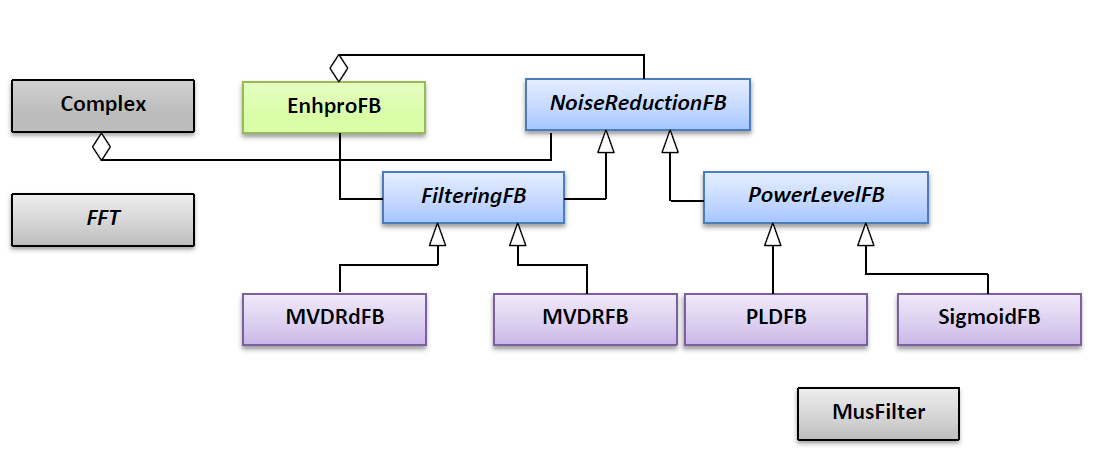
\includegraphics[width=0.9\textwidth]{framehier.png}
  \caption{Relationships for \emph{frame-based} operation mode.}
  \label{fh}
\end{center}
\end{figure}

\begin{figure} [!ht]
\begin{center}
  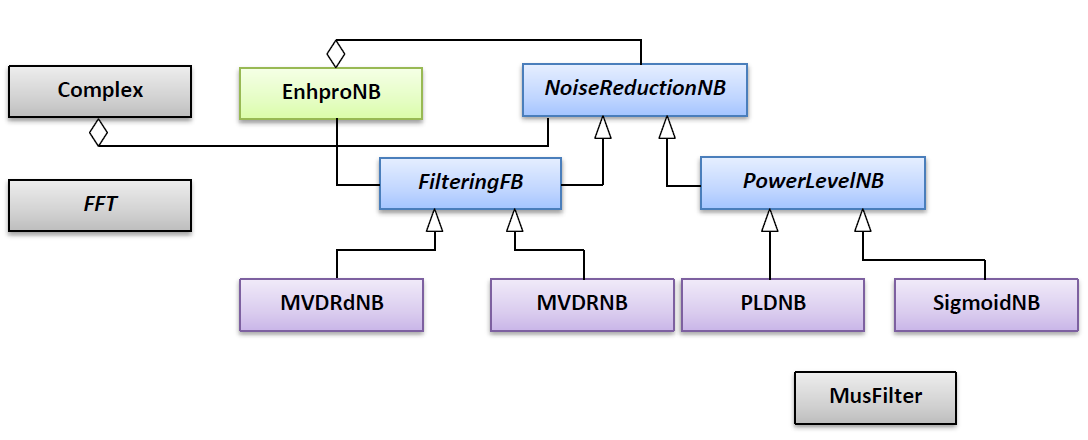
\includegraphics[width=0.9\textwidth]{notehier.png}
  \caption{Relationships for \emph{note-based} operation mode.}
  \label{nh}
\end{center}
\end{figure}

Abstract classes are marked in blue and have italic font. Superclasses are marked in blue, and common to all packages classes are marked in black. Purple colour indicates classes which must be used for algorithm implementation. \texttt{Enhpro} class which implements Overlap-Add method is colored blue.

Regarding relationships among classes, inheritance is symbolized by a white arrowhead. An example is given by \texttt{Filtering} y \texttt{PowerLevel} classes with \texttt{NoiseReduction}. A white diamond indicates one or more objects from this class are used by another class (aggregation relationship). 

\section{Classes}

\subsection{Complex}

\subsubsection*{Identification}

In this subsection (along the entire document) the package hierarchy preceding every class is included, as well as the entire name for the class, as it follows:
\begin{shaded}
\begin{center}
package1.package2.ClassName $>>>$ Class name with identifiers
\end{center}
\end{shaded}

speech.common.Complex $>>>$ public class Complex extends java.lang.Object

\subsubsection*{Class Overview}

Complex is a class that represents a complex number. It includes real and imaginary parts (the complex number in its canonical form), and the main arithmetic.

\subsubsection*{Constructor Summary}

\begin{longtable}{|p{12cm}|}
\hline
\textbf{Constructor and Description}\\
\hline
\textbf{public Complex ()}\\
Default constructor.\\
\hline
\textbf{public Complex (double real\_part, double imaginary\_part)}\\
Constructor with parameters.\\
\hline
\end{longtable}

\subsubsection*{Method Summary}

\begin{longtable}{|p{4cm}|p{8cm}|}
\hline
\textbf{Modifier and Type} & \textbf{Method and Description}\\
\hline
public double & \textbf{getReal()}\\
&Returns the real part.\\
\hline
public double & \textbf{getImag()}\\
&Returns the imaginary part.\\
\hline
public Complex & \textbf{conjugated()}\\
&Returns the conjugate.\\
\hline
public Complex & \textbf{opposite()}\\
&Returns the opposite.\\
\hline
public double & \textbf{module()}\\
&Returns the module.\\
\hline
public double & \textbf{phase()}\\
&Returns the phase.\\
\hline
public Complex & \textbf{modToComp(double mod, double phase)}\\
&Returns a complex number from its module and phase.\\
\hline
public Complex & \textbf{addition(Complex n)}\\
&Returns the addition between complex number and given complex one.\\
\hline
public Complex & \textbf{addition(double n)}\\
&Returns the addition between complex number and given real one.\\
\hline
public Complex & \textbf{subtraction(Complex n)}\\
&Returns the subtraction between complex number and given complex one.\\
\hline
public Complex & \textbf{product(Complex n)}\\
&Returns the product between complex number and given complex one.\\
\hline
public Complex & \textbf{product(double n)}\\
&Returns the product between complex number and given complex one.\\
\hline
public Complex & \textbf{division(Complex n)}\\
&Returns the quotient between complex number and given complex one.\\
\hline
public Complex & \textbf{division(double n)}\\
&Returns the quotient between complex number and given real one.\\
\hline
public String & \textbf{toString()}\\
&Writes the complex number as a string.\\
\hline
\end{longtable}

\subsubsection*{Fields Detail}

\begin{longtable}{|p{4cm}|p{8cm}|}
\hline
\textbf{Modifier and Type} & \textbf{Field and Description}\\
\hline
private final double & \textbf{real}\\
&The real part of the complex number. Default 0.\\
\hline
private final double & \textbf{imaginary}\\
&The imaginary part of the complex number. Default 0.\\
\hline
\end{longtable}

\subsubsection*{Constructor Detail}

\begin{longtable}{|p{12cm}|}
\hline
\textbf{public Complex ()}\\
\hline
Creates a new complex number whose real and imaginary parts are 0.\\
\hline
\end{longtable}

\begin{longtable}{|p{12cm}|}
\hline
\textbf{public Complex (double real\_part, double imaginary\_part)}\\
\hline
Creates a new complex number with given real and imaginary parts.\\
\textbf{\textcolor{gray45}{Parameters:}}\\
\emph{real\_part:} real part of the complex number.\\
\emph{imag\_part:} imaginary part of the complex number.\\
\hline
\end{longtable}

\subsubsection*{Method Detail}

\begin{longtable}{|p{12cm}|}
\hline
\textbf{public double getReal()}\\
\hline
Obtains the real part of the complex number.\\
\textbf{\textcolor{gray45}{Returns:}}\\
the value of field real.\\
\hline
\end{longtable}

\begin{longtable}{|p{12cm}|}
\hline
\textbf{public double getImag()}\\
\hline
Obtains the imaginary part of the complex number.\\
\textbf{\textcolor{gray45}{Returns:}}\\
the value of field imag.\\
\hline
\end{longtable}

 \

\begin{longtable}{|p{12cm}|}
\hline
\textbf{public Complex conjugated()}\\
\hline
Obtains the conjugate of the complex number.\\
\textbf{\textcolor{gray45}{Returns:}}\\
a Complex with the same real part and opposite imaginary part.\\
\hline
\end{longtable}

\begin{longtable}{|p{12cm}|}
\hline
\textbf{public Complex opposite()}\\
\hline
Obtains the opposite complex number.\\
\textbf{\textcolor{gray45}{Returns:}}\\
a Complex with opposite real and imaginary parts.\\
\hline
\end{longtable}

\begin{longtable}{|p{12cm}|}
\hline
\textbf{public double module()}\\
\hline
Obtains the module of the complex number.\\
\textbf{\textcolor{gray45}{Returns:}}\\
a double precision value of the module.\\
\hline
\end{longtable}

\begin{longtable}{|p{12cm}|}
\hline
\textbf{public double phase()}\\
\hline
Obtains the phase of the complex number.\\
\textbf{\textcolor{gray45}{Returns:}}\\
a double precision value of the phase.\\
\hline
\end{longtable}

\begin{longtable}{|p{12cm}|}
\hline
\textbf{public Complex modToComp(double mod, double phase)}\\
\hline
Obtains a new complex number from its module and phase values.\\
\textbf{\textcolor{gray45}{Parameters:}}\\
\emph{mod:} the module of the complex number.\\
\emph{phase:} the phase of the complex number.\\
\textbf{\textcolor{gray45}{Returns:}}\\
a Complex number in the canonical form.\\
\hline
\end{longtable}

\begin{longtable}{|p{12cm}|}
\hline
\textbf{public Complex addition(Complex n)}\\
\hline
Adds the complex number with given complex one.\\
\textbf{\textcolor{gray45}{Parameters:}}\\
\emph{n:} a Complex number.\\
\textbf{\textcolor{gray45}{Returns:}}\\
a Complex sum of this complex number and another complex one.\\
\hline
\end{longtable}

\begin{longtable}{|p{12cm}|}
\hline
\textbf{public Complex addition(double n)}\\
\hline
Adds the complex number with given real one.\\
\textbf{\textcolor{gray45}{Parameters:}}\\
\emph{n:} a real number.\\
\textbf{\textcolor{gray45}{Returns:}}\\
a Complex sum of this complex number and a real one.\\
\hline
\end{longtable}

\begin{longtable}{|p{12cm}|}
\hline
\textbf{public Complex subtraction(Complex n)}\\
\hline
Substracts from the complex number the given one.\\
\textbf{\textcolor{gray45}{Parameters:}}\\
\emph{n:} a complex number.\\
\textbf{\textcolor{gray45}{Returns:}}\\
a Complex subtraction of this complex number and given complex one.\\
\hline
\end{longtable}

\begin{longtable}{|p{12cm}|}
\hline
\textbf{public Complex product(Complex n)}\\
\hline
Multiplies the complex number by the given complex one.\\
\textbf{\textcolor{gray45}{Parameters:}}\\
\emph{n:} a complex number.\\
\textbf{\textcolor{gray45}{Returns:}}\\
a Complex product of this complex number and given complex one.\\
\hline
\end{longtable}

\begin{longtable}{|p{12cm}|}
\hline
\textbf{public Complex product(double n)}\\
\hline
Multiplies the complex number by the given real one.\\
\textbf{\textcolor{gray45}{Parameters:}}\\
\emph{n:} a real number.\\
\textbf{\textcolor{gray45}{Returns:}}\\
a Complex product of this complex number and given real one.\\
\hline
\end{longtable}

\begin{longtable}{|p{12cm}|}
\hline
\textbf{public Complex division(Complex n) throws ArithmeticException}\\
\hline
Divides the complex number by the given complex one.\\
\textbf{\textcolor{gray45}{Parameters:}}\\
\emph{n:} a complex number.\\
\textbf{\textcolor{gray45}{Returns:}}\\
a Complex quotient of this complex number and given complex one.\\
\textbf{\textcolor{gray45}{Throws:}}\\
\emph{ArithmeticException:} if the parameter n is equal to zero.\\
\hline
\end{longtable}

\begin{longtable}{|p{12cm}|}
\hline
\textbf{public Complex division(double n) throws ArithmeticException}\\
\hline
Divides the complex number by the given real one.\\
\textbf{\textcolor{gray45}{Parameters:}}\\
\emph{n:} a real number.\\
\textbf{\textcolor{gray45}{Returns:}}\\
a Complex quotient of this complex number and given real one.\\
\textbf{\textcolor{gray45}{Throws:}}\\
\emph{ArithmeticException:} if the parameter n is equal to zero.\\
\hline
\end{longtable}

\begin{longtable}{|p{12cm}|}
\hline
\textbf{public String toString()}\\
\hline
Writes the complex number as follows: real + imag i.\\
\textbf{\textcolor{gray45}{Returns:}}\\
a string with the complex number in canonical form.\\
\hline
\end{longtable}

\subsection{FFT}

\subsubsection*{Identification}

speech.common.FFT $>>>$ public abstract class FFT extends java.lang.Object

\subsubsection*{Class Overview}

FFT is an abstract class that includes a series of algorithms for converting signals from time domain to frequency domain and vice versa, and convolving two signals.

\subsubsection*{Constructor Summary}

Class FFT has no constructors.

\subsubsection*{Method Summary}

\begin{longtable}{|p{4cm}|p{8cm}|}
\hline
\textbf{Modifier and Type} & \textbf{Method and Description}\\
\hline
public static Complex[] & \textbf{fft(Complex[] signal, int M)}\\
&Returns the FFT of signal.\\
\hline
public static Complex[] & \textbf{ifft(Complex[] sfreq, int M)}\\
&Returns the IFFT of signal.\\
\hline
public static double[] & \textbf{convolution(double[] signal1, double[] signal2)}\\
&Returns the convolution between the 2 signals.\\
\hline
\end{longtable}

\subsubsection*{Fields Detail}

This class has no fields.

\subsubsection*{Method Detail}

\begin{longtable}{|p{12cm}|}
\hline
\textbf{public static Complex[] fft(Complex[] signal, int M)}\\
\hline
Obtains the Fast Fourier Transform of signal, with M the number of samples.\\
\textbf{\textcolor{gray45}{Parameters:}}\\
\emph{signal:} a Complex signal in time domain.\\
\emph{M:} number of samples for the transform.\\
\textbf{\textcolor{gray45}{Returns:}}\\
a Complex vector result of the FFT.\\
\hline
\end{longtable}

\begin{longtable}{|p{12cm}|}
\hline
\textbf{public static Complex[] ifft(Complex[] sfreq, int M)}\\
\hline
Obtains the Inverse Fast Fourier Transform of sfreq, with M the number of samples.\\
\textbf{\textcolor{gray45}{Parameters:}}\\
\emph{sfreq:} a Complex signal in frequency domain.\\
\emph{M:} number of samples for the transform.\\
\textbf{\textcolor{gray45}{Returns:}}\\
a Complex vector result of the IFFT.\\
\hline
\end{longtable}

\begin{longtable}{|p{12cm}|}
\hline
\textbf{public static double[] convolution(double[] signal1, double[] signal2)}\\
\hline
Obtains the convolution between signal1 and signal2.\\
\textbf{\textcolor{gray45}{Parameters:}}\\
\emph{signal1:} a double-precision float signal.\\
\emph{signal2:} another double-precision float signal.\\
\textbf{\textcolor{gray45}{Returns:}}\\
a double vector result of the convolution, with number of samples sum of signal1 and signal2 lengths.\\
\hline
\end{longtable}

\subsection{MusFilter}

\subsubsection*{Identification}

speech.common.MusFilter $>>>$ public class MusFilter extends java.lang.Object

\subsubsection*{Class Overview}

MusFilter is the class that implements musical noise reduction method.

\subsubsection*{Constructor Summary}

\begin{longtable}{|p{12cm}|}
\hline
\textbf{Constructor and Description}\\
\hline
\textbf{public MusFilter ()}\\
Default constructor.\\
\hline
\textbf{public MusFilter(double Eu\_def, int PHIu\_def, int f0u\_def, int Fsu\_def)}\\
Constructor with user-defined parameters.\\
\hline
\end{longtable}

\subsubsection*{Method Summary}

\begin{longtable}{|p{4cm}|p{8cm}|}
\hline
\textbf{Modifier and Type} & \textbf{Method and Description}\\
\hline
public double[][] & \textbf{musfilter(Complex[][] Xf1, double[][] G0)}\\
&Returns modified gains to suppress musical noise.\\
\hline
\end{longtable}

\subsubsection*{Fields Detail}

\begin{longtable}{|p{4cm}|p{8cm}|}
\hline
\textbf{Modifier and Type} & \textbf{Field and Description}\\
\hline
private final double & \textbf{Eth}\\
&Threshold for low-SNR detection. Default 0.4.\\
\hline
private final int & \textbf{f0}\\
&Frequency below which musical noise supresion is performed. Default 1000.\\
\hline
private final int & \textbf{Fs}\\
&Sampling frequency. Default 8000.\\
\hline
private final int & \textbf{PHI}\\
&Scaling factor for the maximum degree of smoothing in filtering. Default 10.\\
\hline
\end{longtable}

\subsubsection*{Constructor Detail}

\begin{longtable}{|p{12cm}|}
\hline
\textbf{public MusFilter ()}\\
\hline
Creates a new MusFilter object which fields initialized to default value.\\
\hline
\end{longtable}

\begin{longtable}{|p{12cm}|}
\hline
\textbf{public MusFilter(double Eu\_def, int PHIu\_def, int f0u\_def, int Fsu\_def)}\\
\hline
Creates a new MusFilter object with given values for fields.\\
\textbf{\textcolor{gray45}{Parameters:}}\\
\emph{Eu\_def:} user-defined low-SNR detection threshold.\\
\emph{PHIu\_def:} user-defined scaling factor for smoothing.\\
\emph{f0u\_def:} user-defined threshold frequency for musical noise reduction.\\
\emph{Fsu\_def:} user-defined sampling frequency.\\
\hline
\end{longtable}

\subsubsection*{Method Detail}

\begin{longtable}{|p{12cm}|}
\hline
\textbf{public double[][] musfilter(Complex[][] Xf1, double[][] G0)}\\
\hline
Modifies gains to suppress musical noise, from low-SNR detection and adaptive smoothing.\\
\textbf{\textcolor{gray45}{Parameters:}}\\
\emph{Xf1:} signal frames in frequency domain.\\
\emph{G0:} initial frame gains.\\
\textbf{\textcolor{gray45}{Returns:}}\\
a double matrix with modified frame gains.\\
\hline
\end{longtable}

\subsection{EnhproFB}

\subsubsection*{Identification}

speech.common.EnhproFB $>>>$ public class EnhproFB extends java.lang.Object

\subsubsection*{Class Overview}

EnhproFB deals with implementing Overlap-Add method, for \emph{frame-based} operation mode. 

\subsubsection*{Constructor Summary}

\begin{longtable}{|p{12cm}|}
\hline
\textbf{Constructor and Description}\\
\hline
\textbf{public EnhproFB ()}\\
Default constructor.\\
\hline
\textbf{public EnhproFB(int Freq, int Lframe, int Ltransf)}\\
Constructor with user-defined parameters.\\
\hline
\end{longtable}

\subsubsection*{Method Summary}

\begin{longtable}{|p{4cm}|p{8cm}|}
\hline
\textbf{Modifier and Type} & \textbf{Method and Description}\\
\hline
public void & \textbf{preProcessing(short[] x1, short[] x2)}\\
&Converts time domain frames to frequency domain.\\
\hline
public void & \textbf{postProcessing(Complex[][] Xf, boolean end)}\\
&Converts frequency domain frames to time domain.\\
\hline
public int & \textbf{getFs()}\\
&Returns sampling frequency.\\
\hline
public int & \textbf{getM()}\\
&Returns number of samples for FFT.\\
\hline
private static Complex[] & \textbf{obtCol(Complex[][] mat, int index)}\\
&Returns a column from 'mat' matrix.\\
\hline
\end{longtable}

\subsubsection*{Fields Detail}

\begin{longtable}{|p{4cm}|p{8cm}|}
\hline
\textbf{Modifier and Type} & \textbf{Field and Description}\\
\hline
private boolean & \textbf{initPre}\\
&Indicates if it is first iteration of pre-processing (true), or not (false). Default true.\\
\hline
private boolean & \textbf{initPost}\\
&Indicates if it is first iteration of post-processing (true), or not (false). Default true.\\
\hline
private int & \textbf{L}\\
&Frame length in time domain. Default 160.\\
\hline
private int & \textbf{Os}\\
&Overlap length (half of frame length). Default 80.\\
\hline
private int & \textbf{Fs}\\
&Sampling frequency. Default 8000.\\
\hline
private int & \textbf{M}\\
&Number of samples for FFT. Default 256.\\
\hline
private double & \textbf{a0}\\
&Parameter for Hann window. Default 0.5.\\
\hline
private double & \textbf{a1}\\
&Parameter for Hann window. Default 0.5\\
\hline
private double[] & \textbf{hann}\\
&Hann window, length L.\\
\hline
private short[] & \textbf{ov1}\\
&Overlap samples for primary microphone signal, lenght Os.\\
\hline
private short[] & \textbf{ov2}\\
&Overlap samples for secondary microphone signal, length Os.\\
\hline
private Complex[] & \textbf{frame1}\\
&Current frame for primary microphone signal, length L.\\
\hline
private Complex[] & \textbf{frame2}\\
&Current frame for secondary microphone signal, length L.\\
\hline
Complex[] & \textbf{Xf1}\\
&Frequency domain conversion for current primary microphone frame.\\
\hline
Complex[] & \textbf{Xf2}\\
&Frequency domain conversion for current secondary microphone frame.\\
\hline
Complex[] & \textbf{Xcomplex}\\
&Reconstructed frame.\\
\hline
short[] & \textbf{Xrec}\\
&Reconstructed frame, PCM encoding.\\
\hline
\end{longtable}

\subsubsection*{Constructor Detail}

\begin{longtable}{|p{12cm}|}
\hline
\textbf{public EnhproFB ()}\\
\hline
Creates a new EnhproFB object with default parameters for fields.\\
\hline
\end{longtable}

\begin{longtable}{|p{12cm}|}
\hline
\textbf{public EnhproFB(int Freq, int Lframe, int Ltransf) throws InvalidFrequencyException, InvalidParametersException}\\
\hline
Creates a new EnhproFB object with given values for fields. Other fields has default values.\\
\textbf{\textcolor{gray45}{Parameters:}}\\
\emph{Freq:} user-defined sampling frequency.\\
\emph{Lframe:} user-defined frame length.\\
\emph{Ltransf:} user-defined number of samples for FFT.\\
\textbf{\textcolor{gray45}{Throws:}}\\
\emph{InvalidFrequencyException:} if frequency is different of 8000, 16000, 44100.\\
\emph{InvalidParametersException:} if frame length is greater than number of samples for FFT.\\
\hline
\end{longtable}

\subsubsection*{Method Detail}

\begin{longtable}{|p{12cm}|}
\hline
\textbf{public void preProcessing(short[] x1, short[] x2)}\\
\hline
Convert frame in time domain to frequency domain, with windowing and 50\% overlap.\\
\textbf{\textcolor{gray45}{Parameters:}}\\
\emph{x1:} signal frame from primary microphone.\\
\emph{x2:} signal frame from secondary microphone.\\
\hline
\end{longtable}

\begin{longtable}{|p{12cm}|}
\hline
\textbf{public void postProcessing(Complex[][] Xf, boolean end)}\\
\hline
Convert frame in frequency domain to time domain, applying Overlap-Add method.\\
\textbf{\textcolor{gray45}{Parameters:}}\\
\emph{Xf:} signal frame in frequency domain.\\
\emph{end:} indicates if frame is the last one (true) or not (false).\\
\hline
\end{longtable}

\begin{longtable}{|p{12cm}|}
\hline
\textbf{public int getFs ()}\\
\hline
Obtains sampling frequency.\\
\textbf{\textcolor{gray45}{Returns:}}\\
integer field Fs.\\
\hline
\end{longtable}

\begin{longtable}{|p{12cm}|}
\hline
\textbf{public int getM ()}\\
\hline
Obtains number of samples for FFT.\\
\textbf{\textcolor{gray45}{Returns:}}\\
integer field M.\\
\hline
\end{longtable}

\begin{longtable}{|p{12cm}|}
\hline
\textbf{private static Complex[] obtCol (Complex[][] mat, int index)}\\
\hline
Obtains the given index column from 'mat'.\\
\textbf{\textcolor{gray45}{Parameters:}}\\
\emph{mat:} a Complex matrix.\\
\emph{index:} index to the column to extract.\\
\textbf{\textcolor{gray45}{Returns:}}\\
a vector with the column of given index.\\
\hline
\end{longtable}

\subsection{NoiseReductionFB}

\subsubsection*{Identification}

speech.common.NoiseReductionFB $>>>$ public abstract class NoiseReductionFB extends java.lang.Object

\subsubsection*{Direct Known Subclasses}

FilteringFB

PowerLevelFB

\subsubsection*{Class Overview}

NoiseReductionFB is the abstract superclass which groups all kinds of algorithms that work in \emph{frame-based} operation mode.

\subsubsection*{Constructor Summary}

\begin{longtable}{|p{12cm}|}
\hline
\textbf{Constructor and Description}\\
\hline
\textbf{NoiseReductionFB ()}\\
Default constructor.\\
\hline
\end{longtable}

\subsubsection*{Method Summary}

\begin{longtable}{|p{4cm}|p{8cm}|}
\hline
\textbf{Modifier and Type} & \textbf{Method and Description}\\
\hline
void & \textbf{initProcessing(short[] x1, short[] x2)}\\
&Performs pre-processing of the frames.\\
\hline
\end{longtable}

\subsubsection*{Fields Detail}

\begin{longtable}{|p{4cm}|p{8cm}|}
\hline
\textbf{Modifier and Type} & \textbf{Field and Description}\\
\hline
EnhproFB & \textbf{freq\_time}\\
&EnhproFB class object for processing.\\
\hline
Complex[][] & \textbf{Xf}\\
&Processed signal in frequency domain.\\
\hline
\end{longtable}

\subsubsection*{Constructor Detail}

\begin{longtable}{|p{12cm}|}
\hline
\textbf{NoiseReductionFB ()}\\
\hline
Creates a new NoiseReductionFB object with initializes EnhproFB object.\\
\hline
\end{longtable}

\begin{longtable}{|p{12cm}|}
\hline
\textbf{NoiseReductionFB (int Freq, int Lframe, int Ltransf) throws EnhproFB.InvalidFrequencyException, EnhproFB.InvalidParametersException}\\
\hline
Creates a new NoiseReductionFB object with initializes EnhproFB object with given parameters.\\
\textbf{\textcolor{gray45}{Parameters:}}\\
\emph{Freq:} user-defined sampling frequency.\\
\emph{Lframe:} user-defined frame length.\\
\emph{Ltransf:} user-defined number of samples for FFT.\\
\textbf{\textcolor{gray45}{Throws:}}\\
\emph{InvalidFrequencyException:} if frequency is different of 8000, 16000, 44100.\\
\emph{InvalidParametersException:} if frame length is greater than number of samples for FFT.\\
\hline
\end{longtable}

\subsubsection*{Method Detail}

\begin{longtable}{|p{12cm}|}
\hline
\textbf{void initProcessing(short[] x1, short[] x2)}\\
\hline
Calls pre-processing EnhproFB class method to convert frames to frequency domain. Initializes processed frame Xf.\\
\textbf{\textcolor{gray45}{Parameters:}}\\
\emph{x1:} signal frame from primary microphone.\\
\emph{x2:} signal frame from secondary microphone.\\
\hline
\end{longtable}

\subsection{FilteringFB}

\subsubsection*{Identification}

speech.common.FilteringFB $>>>$ public abstract class FilteringFB extends NoiseReductionFB

\subsubsection*{Direct Known Subclasses}

MVDRFB

MVDRdFB

\subsubsection*{Class Overview}

FilteringFB is the abstract superclass which groups algorithms based on filtering incoming signals that work in \emph{frame-based} operation mode.

\subsubsection*{Constructor Summary}

\begin{longtable}{|p{12cm}|}
\hline
\textbf{Constructor and Description}\\
\hline
\textbf{FilteringFB ()}\\
Default constructor.\\
\hline
\textbf{FilteringFB (int Freq, int Lframe, int Ltransf) throws EnhproFB.InvalidFrequencyException, EnhproFB.InvalidParametersException}\\
Constructor with user-defined parameters.\\
\hline
\end{longtable}

\subsubsection*{Method Summary}

\begin{longtable}{|p{4cm}|p{8cm}|}
\hline
\textbf{Modifier and Type} & \textbf{Method and Description}\\
\hline
void & \textbf{initProcessing(short[] x1, short[] x2)}\\
&Performs pre-processing of the frames.\\
\hline
short[] & \textbf{obtainXrec(boolean end)}\\
&Converts frequency domain frames to time domain.\\
\hline
public void & \textbf{changeAtFactor(double[][] newAt)}\\
&Change attenuation factor between microphones.\\
\hline
public void & \textbf{changeDel(double newDel)}\\
&Change delay between microphones.\\
\hline
void & \textbf{meanCorr(double[] v1, double v2[], int end)}\\
&Returns the mean of the correlation between the first samples of vectors, given by end.\\
\hline
\end{longtable}

\subsubsection*{Fields Detail}

\begin{longtable}{|p{4cm}|p{8cm}|}
\hline
\textbf{Modifier and Type} & \textbf{Field and Description}\\
\hline
double[][] & \textbf{at}\\
&Attenuation factor (magnitude) between microphones, for each frequency bin. Default: see \label{attabla}.\\
\hline
private double & \textbf{del}\\
&Delay between microphones, in samples. Default: 2.2745 samples.\\
\hline
final Complex[] & \textbf{d}\\
&Steering vector estimation.\\
\hline
final double[] & \textbf{f}\\
&Frequency vector for each bin.\\
\hline
Complex[] & \textbf{w}\\
&Weight vector.\\
\hline
private double[][] & \textbf{phases}\\
&Phases from primary channel frame.\\
\hline
\end{longtable}

\begin{longtable}{|p{12cm}|}
\hline
\textbf{Fields inherited from speech.frame.NoiseReductionFB: }\\
\hline
freq\_time, Xf\\
\hline
\end{longtable}

\subsubsection*{Constructor Detail}

\begin{longtable}{|p{12cm}|}
\hline
\textbf{FilteringFB ()}\\
\hline
Creates a new FilteringFB object. Initializes vector dimensions and frequency and steering vector values.\\
\hline
\end{longtable}

\begin{longtable}{|p{12cm}|}
\hline
\textbf{FilteringFB (int Freq, int Lframe, int Ltransf) throws EnhproFB.InvalidFrequencyException, EnhproFB.InvalidParametersException}\\
\hline
Creates a new FilteringFB object with user-defined parameters. Initializes vector dimensions and frequency and steering vector values.\\
\textbf{\textcolor{gray45}{Parameters:}}\\
\emph{Freq:} user-defined sampling frequency.\\
\emph{Lframe:} user-defined frame length.\\
\emph{Ltransf:} user-defined number of samples for FFT.\\
\textbf{\textcolor{gray45}{Throws:}}\\
\emph{InvalidFrequencyException:} if frequency is different of 8000, 16000, 44100.\\
\emph{InvalidParametersException:} if frame length is greater than number of samples for FFT.\\
\hline
\end{longtable}

\subsubsection*{Method Detail}

\begin{longtable}{|p{12cm}|}
\hline
\textbf{void initProcessing(short[] x1, short[] x2)}\\
\hline
Calls superclass same name method and initializes phases vector dimension.\\
\textbf{\textcolor{gray45}{Overrides:}}\\
method initProcessing in class NoiseReductionFB.
\textbf{\textcolor{gray45}{Parameters:}}\\
\emph{x1:} signal frame from primary microphone.\\
\emph{x2:} signal frame from secondary microphone.\\
\hline
\end{longtable}

\begin{longtable}{|p{12cm}|}
\hline
\textbf{short[] obtainXrec(boolean end)}\\
\hline
Adds first-channel frame phases to reconstructed frame in frequency domain. Gets the frame back in time domain.\\
\textbf{\textcolor{gray45}{Parameters:}}\\
\emph{end:} indicates if frame is the last one (true) or not (false).\\
\textbf{\textcolor{gray45}{Returns:}}\\
a short precision frame in time domain.\\
\hline
\end{longtable}

\begin{longtable}{|p{12cm}|}
\hline
\textbf{public static void \emph{changeAt}(double[][] newAt)}\\
\hline
Change the attenuation factor between microphones by a new one. It must have a size of $[\frac{M}{2}+1][2]$, being M the size of FFT.\\
\textbf{\textcolor{gray45}{Parameters:}}\\
\emph{newAt:} the new attenuation factor.\\
\hline
\end{longtable}

\begin{longtable}{|p{12cm}|}
\hline
\textbf{public static void \emph{changeDel}(double newDel)}\\
\hline
Change the delay between microphones by a new one.\\
\textbf{\textcolor{gray45}{Parameters:}}\\
\emph{newDel:} the new delay in samples.\\
\hline
\end{longtable}

\begin{longtable}{|p{12cm}|}
\hline
\textbf{double meanCorr(double[] v1, double[] v2, int end)}\\
\hline
Calculates the mean of correlation between the number of samples of v1 and v2 given by end.\\
\textbf{\textcolor{gray45}{Parameters:}}\\
\emph{v1:} the first vector.\\
\emph{v2:} the second vector.\\
\emph{end:} the number of treated samples.\\
\hline
\end{longtable}


\subsection{PowerLevelFB}

\subsubsection*{Identification}

speech.common.PowerLevelFB $>>>$ public abstract class PowerLevelFB extends NoiseReductionFB

\subsubsection*{Direct Known Subclasses}

PLDFB

SigmoidFB

\subsubsection*{Class Overview}

PowerLevelFB is the abstract superclass which groups algorithms based on power level differences between dual-microphone signals that work in \emph{frame-based} operation mode.

\subsubsection*{Constructor Summary}

\begin{longtable}{|p{12cm}|}
\hline
\textbf{Constructor and Description}\\
\hline
\textbf{PowerLevelFB (boolean noise)}\\
Default constructor.\\
\hline
\textbf{PowerLevelFB (boolean noise, int Freq, int Lframe, int Ltransf) throws EnhproFB.InvalidFrequencyException, EnhproFB.InvalidParametersException}\\
Constructor with user-defined parameters.\\
\hline
\end{longtable}

\subsubsection*{Method Summary}

\begin{longtable}{|p{4cm}|p{8cm}|}
\hline
\textbf{Modifier and Type} & \textbf{Method and Description}\\
\hline
void & \textbf{initProcessing(short[] x1, short[] x2)}\\
&Performs pre-processing of the frames.\\
\hline
short[] & \textbf{obtainXrec(boolean end)}\\
&Converts frequency domain frames to time domain.\\
\hline
private void & \textbf{rec(double[][] Gan, Complex[][] Sfreq)}\\
&Applies spectral gains to frames in frequency domain.\\
\hline
\end{longtable}

\subsubsection*{Fields Detail}

\begin{longtable}{|p{4cm}|p{8cm}|}
\hline
\textbf{Modifier and Type} & \textbf{Field and Description}\\
\hline
final double & \textbf{a1}\\
&Forgetting factor for PSD calculation. Default 0.9.\\
\hline
final boolean & \textbf{WN}\\
&Indicates if musical noise reduction is applied (true) or not (false). Default false.\\
\hline
double[][] & \textbf{PSD1}\\
&Power Spectral Density of primary channel.\\
\hline
double[][] & \textbf{PSD2}\\
&Power Spectral Density of secondary channel.\\
\hline
double[][] & \textbf{G}\\
&Spectral gains.\\
\hline
\end{longtable}

\begin{longtable}{|p{12cm}|}
\hline
\textbf{Fields inherited from speech.frame.NoiseReductionFB: }\\
\hline
freq\_time, Xf\\
\hline
\end{longtable}

\subsubsection*{Constructor Detail}

\begin{longtable}{|p{12cm}|}
\hline
\textbf{PowerLevelFB (boolean noise)}\\
\hline
Creates a new PowerLevelFB object. Initializes PSDs vector dimensions and default fields, and WN with the value of noise parameter.\\
\textbf{\textcolor{gray45}{Parameters:}}\\
\emph{noise:} indicates if musical noise reduction is used (true), or not (false).\\
\hline
\end{longtable}

\begin{longtable}{|p{12cm}|}
\hline
\textbf{PowerLevelFB (boolean noise, int Freq, int Lframe, int Ltransf) throws EnhproFB.InvalidFrequencyException, EnhproFB.InvalidParametersException}\\
\hline
Creates a new PowerLevelFB object, with parameters above. Initializes PSDs vector dimensions and default fields, and WN with the value of noise parameter.\\
\textbf{\textcolor{gray45}{Parameters:}}\\
\emph{noise:} indicates if musical noise reduction is used (true), or not (false).\\
\emph{Freq:} user-defined sampling frequency.\\
\emph{Lframe:} user-defined frame length.\\
\emph{Ltransf:} user-defined number of samples for FFT.\\
\textbf{\textcolor{gray45}{Throws:}}\\
\emph{InvalidFrequencyException:} if frequency is different of 8000, 16000, 44100.\\
\emph{InvalidParametersException:} if frame length is greater than number of samples for FFT.\\
\hline
\end{longtable}

\subsubsection*{Method Detail}

\begin{longtable}{|p{12cm}|}
\hline
\textbf{void initProcessing(short[] x1, short[] x2)}\\
\hline
Calls superclass same name method and initializes spectral gains vector dimensions.\\
\textbf{\textcolor{gray45}{Overrides:}}\\
method initProcessing in class NoiseReductionFB.
\textbf{\textcolor{gray45}{Parameters:}}\\
\emph{x1:} signal frame from primary microphone.\\
\emph{x2:} signal frame from secondary microphone.\\
\hline
\end{longtable}

\begin{longtable}{|p{12cm}|}
\hline
\textbf{short[] obtainXrec(boolean end)}\\
\hline
Reconstructs frame from spectral gains in frequency domain. Gets the frame back in time domain.\\
\textbf{\textcolor{gray45}{Parameters:}}\\
\emph{end:} indicates if frame is the last one (true) or not (false).\\
\textbf{\textcolor{gray45}{Returns:}}\\
a frame in time domain, in short integer format.\\
\hline
\end{longtable}

\begin{longtable}{|p{12cm}|}
\hline
\textbf{private void rec(double[][] Gan, Complex[][] Sfreq)}\\
\hline
Applies spectral gains to frames in frequency domain, product through frequency bins.\\
\textbf{\textcolor{gray45}{Parameters:}}\\
\emph{Gan:} spectral gains.\\
\emph{Sfreq:} frames in frequency domain.\\
\hline
\end{longtable}

\subsection{MVDRFB}

\subsubsection*{Identification}

speech.common.MVDRFB $>>>$ public class MVDRFB extends FilteringFB

\subsubsection*{Class Overview}

MVDRFB is the class which implements MVDR algorithm regardless of the delay between channels, for \emph{frame-based} operation mode.

\subsubsection*{Constructor Summary}

\begin{longtable}{|p{12cm}|}
\hline
\textbf{Constructor and Description}\\
\hline
\textbf{public MVDRFB ()}\\
Default constructor.\\
\hline
\textbf{public MVDRFB (int Freq, int Lframe, int Ltransf) throws EnhproFB.InvalidFrequencyException, EnhproFB.InvalidParametersException}\\
Constructor with user-defined parameters.\\
\hline
\end{longtable}

\subsubsection*{Method Summary}

\begin{longtable}{|p{4cm}|p{8cm}|}
\hline
\textbf{Modifier and Type} & \textbf{Method and Description}\\
\hline
public short[] & \textbf{processing(short[] x1, short[] x2, boolean end) throws ArithmeticException}\\
&Performs processing of the frames according to the MVDR algorithm, without delay.\\
\hline
\end{longtable}

\subsubsection*{Fields Detail}

\begin{longtable}{|p{4cm}|p{8cm}|}
\hline
\textbf{Modifier and Type} & \textbf{Field and Description}\\
\hline
private int & \textbf{count}\\
&Frame counter. Default 0.\\
\hline
private double & \textbf{N1}\\
&Noise samples vector for first channel.\\
\hline
private double & \textbf{N2}\\
&Noise samples vector for second channel.\\
\hline
private double[][] & \textbf{R}\\
&Noise correlation matrix.\\
\hline
\end{longtable}

\begin{longtable}{|p{12cm}|}
\hline
\textbf{Fields inherited from speech.frame.NoiseReductionFB: }\\
\hline
freq\_time, Xf\\
\hline
\end{longtable}

\begin{longtable}{|p{12cm}|}
\hline
\textbf{Fields inherited from speech.frame.FilteringFB: }\\
\hline
at, d, f, w\\
\hline
\end{longtable}

\subsubsection*{Constructor Detail}

\begin{longtable}{|p{12cm}|}
\hline
\textbf{public MVDRFB ()}\\
\hline
Creates a new MVDRFB object. Initializes count to zero and noise sample vector dimensions.\\
\hline
\end{longtable}

\begin{longtable}{|p{12cm}|}
\hline
\textbf{public MVDRFB (int Freq, int Lframe, int Ltransf) throws EnhproFB.InvalidFrequencyException, EnhproFB.InvalidParametersException}\\
\hline
Creates a new MVDRFB object with user-defined parameters. Initializes count to zero and noise sample vector dimensions.\\
\textbf{\textcolor{gray45}{Parameters:}}\\
\emph{Freq:} user-defined sampling frequency.\\
\emph{Lframe:} user-defined frame length.\\
\emph{Ltransf:} user-defined number of samples for FFT.\\
\textbf{\textcolor{gray45}{Throws:}}\\
\emph{InvalidFrequencyException:} if frequency is different of 8000, 16000, 44100.\\
\emph{InvalidParametersException:} if frame length is greater than number of samples for FFT.\\
\hline
\end{longtable}

\subsubsection*{Method Detail}

\begin{longtable}{|p{12cm}|}
\hline
\textbf{public short[] processing(short[] x1, short[] x2, boolean end) throws ArithmeticException}\\
\hline
Applies MVDR algorithm, without delay between channels, to given frames.\\
\textbf{\textcolor{gray45}{Parameters:}}\\
\emph{x1:} signal frame from primary microphone.\\
\emph{x2:} signal frame from secondary microphone.\\
\emph{end:} indicates if frame is the last one (true) or not (false).\\
\textbf{\textcolor{gray45}{Returns:}}\\
a frame in time domain, in short integer format.
\textbf{\textcolor{gray45}{Throws:}}\\
\emph{Arithmetic Exception:} see method division in Complex class.\\
\hline
\end{longtable}

\begin{longtable}{|p{12cm}|}
\hline
\textbf{Methods inherited from speech.frame.FilteringFB: }\\
\hline
initProcessing, obtainXrec, \emph{changeAt}, \emph{changeDel}, meanCorr\\
\hline
\end{longtable}

\subsection{MVDRdFB}

\subsubsection*{Identification}

speech.common.MVDRdFB $>>>$ public class MVDRdFB extends FilteringFB

\subsubsection*{Class Overview}

MVDRdFB is the class which implements MVDR algorithm with delay between microphones, for \emph{frame-based} operation mode.

\subsubsection*{Constructor Summary}

\begin{longtable}{|p{12cm}|}
\hline
\textbf{Constructor and Description}\\
\hline
\textbf{public MVDRdFB ()}\\
Default constructor.\\
\hline
\textbf{public MVDRdFB (int Freq, int Lframe, int Ltransf) throws EnhproFB.InvalidFrequencyException, EnhproFB.InvalidParametersException}\\
Constructor with user-defined parameters.\\
\hline
\end{longtable}

\subsubsection*{Method Summary}

\begin{longtable}{|p{4cm}|p{8cm}|}
\hline
\textbf{Modifier and Type} & \textbf{Method and Description}\\
\hline
public short[] & \textbf{processing(short[] x1, short[] x2, boolean end) throws ArithmeticException}\\
&Performs processing of the frames according to the MVDR algorithm, with delay.\\
\hline
\end{longtable}

\subsubsection*{Fields Detail}

\begin{longtable}{|p{4cm}|p{8cm}|}
\hline
\textbf{Modifier and Type} & \textbf{Field and Description}\\
\hline
private int & \textbf{count}\\
&Frame counter. Default 0.\\
\hline
private double & \textbf{N1}\\
&Noise samples vector for first channel.\\
\hline
private double & \textbf{N2}\\
&Noise samples vector for second channel.\\
\hline
private double[][] & \textbf{R}\\
&Noise correlation matrix.\\
\hline
\end{longtable}

\begin{longtable}{|p{12cm}|}
\hline
\textbf{Fields inherited from speech.frame.NoiseReductionFB: }\\
\hline
freq\_time, Xf\\
\hline
\end{longtable}

\begin{longtable}{|p{12cm}|}
\hline
\textbf{Fields inherited from speech.frame.FilteringFB: }\\
\hline
at, d, f, w\\
\hline
\end{longtable}

\subsubsection*{Constructor Detail}

\begin{longtable}{|p{12cm}|}
\hline
\textbf{public MVDRdFB ()}\\
\hline
Creates a new MVDRdFB object. Initializes count to zero and noise sample vector dimensions.\\
\hline
\end{longtable}

\begin{longtable}{|p{12cm}|}
\hline
\textbf{public MVDRFB (int Freq, int Lframe, int Ltransf) throws EnhproFB.InvalidFrequencyException, EnhproFB.InvalidParametersException}\\
\hline
Creates a new MVDRdFB object with user-defined parameters. Initializes count to zero and noise sample vector dimensions.\\
\textbf{\textcolor{gray45}{Parameters:}}\\
\emph{Freq:} user-defined sampling frequency.\\
\emph{Lframe:} user-defined frame length.\\
\emph{Ltransf:} user-defined number of samples for FFT.\\
\textbf{\textcolor{gray45}{Throws:}}\\
\emph{InvalidFrequencyException:} if frequency is different of 8000, 16000, 44100.\\
\emph{InvalidParametersException:} if frame length is greater than number of samples for FFT.\\
\hline
\end{longtable}

\subsubsection*{Method Detail}

\begin{longtable}{|p{12cm}|}
\hline
\textbf{public short[] processing(short[] x1, short[] x2, boolean end) throws ArithmeticException}\\
\hline
Applies MVDR algorithm taking into account delay between microphones, to given frames.\\
\textbf{\textcolor{gray45}{Parameters:}}\\
\emph{x1:} signal frame from primary microphone.\\
\emph{x2:} signal frame from secondary microphone.\\
\emph{end:} indicates if frame is the last one (true) or not (false).\\
\textbf{\textcolor{gray45}{Returns:}}\\
a frame in time domain, in short integer format.
\textbf{\textcolor{gray45}{Throws:}}\\
\emph{Arithmetic Exception:} see method division in Complex class.\\
\hline
\end{longtable}

\begin{longtable}{|p{12cm}|}
\hline
\textbf{Methods inherited from speech.frame.FilteringFB: }\\
\hline
initProcessing, obtainXrec, \emph{changeAt}, \emph{changeDel}, meanCorr\\
\hline
\end{longtable}

\subsection{PLDFB}

\subsubsection*{Identification}

speech.common.PLDFB $>>>$ public class PLDFB extends PowerLevelFB

\subsubsection*{Class Overview}

PLDFB is the class which implements PLD algorithm, for \emph{frame-based} operation mode.

\subsubsection*{Constructor Summary}

\begin{longtable}{|p{12cm}|}
\hline
\textbf{Constructor and Description}\\
\hline
\textbf{public PLDFB (boolean noise)}\\
Default constructor.\\
\hline
\textbf{public PLDFB (boolean noise, int Freq, int Lframe, int Ltransf, double d) throws EnhproFB.InvalidFrequencyException, EnhproFB.InvalidParametersException}\\
Constructor with user-defined parameters.\\
\hline
\end{longtable}

\subsubsection*{Method Summary}

\begin{longtable}{|p{4cm}|p{8cm}|}
\hline
\textbf{Modifier and Type} & \textbf{Method and Description}\\
\hline
public short[] & \textbf{processing(short[] x1, short[] x2, boolean end)}\\
&Performs processing of the frames according to the PLD algorithm.\\
\hline
private double & \textbf{sinc (double x))}\\
&Returns sinc function of 'x' argument.\\
\hline
private double & \textbf{max (double n1, double n2))}\\
&Returns maximum value of two arguments.\\
\hline
\end{longtable}

\subsubsection*{Fields Detail}

\begin{longtable}{|p{4cm}|p{8cm}|}
\hline
\textbf{Modifier and Type} & \textbf{Field and Description}\\
\hline
private final double & \textbf{a2}\\
&Forgetting factor for updating PSD noise if only noise is present. Default 0.9.\\
\hline
private final double & \textbf{a3}\\
&Forgetting factor for updating PSD noise if speech and noise are present. Default 0.8.\\
\hline
private final double & \textbf{minth}\\
&Minimum PLDNE threshold for distinction only noise. Default 0.2.\\
\hline
private final double & \textbf{maxth}\\
&Maximum PLDNE threshold for distinction only speech. Default 0.8.\\
\hline
private final double & \textbf{dmic}\\
&Distance between microphones. Default 0.1 m.\\
\hline
private final double & \textbf{c}\\
&Sound speed. Default $340 \frac{m}{s}$.\\
\hline
private final double & \textbf{gamma}\\
&Overestimation noise factor. Default 4.\\
\hline
private double[] & \textbf{f}\\
&Frequency vector for each bin.\\
\hline
private double[] & \textbf{Coh}\\
&Coherence function for diffuse noise field.\\
\hline
private double[][] & \textbf{PSD12}\\
&Crossed PSD between channels.\\
\hline
private double[][] & \textbf{PSDr}\\
&Noise PSD estimation.\\
\hline
private double[][] & \textbf{PLDNE}\\
&PLD Noise Estimator (0 indicates speech absence, 1 only speech presence).\\
\hline
private double[][] & \textbf{H12}\\
&Transfer function between channels.\\
\hline
\end{longtable}

\begin{longtable}{|p{12cm}|}
\hline
\textbf{Fields inherited from speech.frame.NoiseReductionFB: }\\
\hline
freq\_time, Xf\\
\hline
\end{longtable}

\begin{longtable}{|p{12cm}|}
\hline
\textbf{Fields inherited from speech.frame.PowerLevelFB: }\\
\hline
WN, a1, PSD1, PSD2, G\\
\hline
\end{longtable}

\subsubsection*{Constructor Detail}

\begin{longtable}{|p{12cm}|}
\hline
\textbf{public PLDFB (boolean noise)}\\
\hline
Creates a new PLDFB object. Initializes fields and vector dimensions. Musical noise reduction is used depending on 'noise' value.\\
\textbf{\textcolor{gray45}{Parameters:}}\\
\emph{noise:} indicates if musical noise reduction is used (true), or not (false).\\
\hline
\end{longtable}

\begin{longtable}{|p{12cm}|}
\hline
\textbf{public PLDFB (boolean noise, int Freq, int Lframe, int Ltransf, double d) throws EnhproFB.InvalidFrequencyException, EnhproFB.InvalidParametersException}\\
\hline
Creates a new PLDFB object with user-defined parameters. Initializes fields and vector dimensions. Musical noise reduction is used depending on 'noise' value.\\
\textbf{\textcolor{gray45}{Parameters:}}\\
\emph{noise:} indicates if musical noise reduction is used (true), or not (false).\\
\emph{Freq:} user-defined sampling frequency.\\
\emph{Lframe:} user-defined frame length.\\
\emph{Ltransf:} user-defined number of samples for FFT.\\
\emph{d:} user-defined distance between microphones.\\
\textbf{\textcolor{gray45}{Throws:}}\\
\emph{InvalidFrequencyException:} if frequency is different of 8000, 16000, 44100.\\
\emph{InvalidParametersException:} if frame length is greater than number of samples for FFT.\\
\hline
\end{longtable}

\subsubsection*{Method Detail}

\begin{longtable}{|p{12cm}|}
\hline
\textbf{public short[] processing(short[] x1, short[] x2, boolean end)}\\
\hline
Applies PLD algorithm to given frames. Uses musical noise reduction depend on constructor parameter.\\
\textbf{\textcolor{gray45}{Parameters:}}\\
\emph{x1:} signal frame from primary microphone.\\
\emph{x2:} signal frame from secondary microphone.\\
\emph{end:} indicates if frame is the last one (true) or not (false).\\
\textbf{\textcolor{gray45}{Returns:}}\\
a frame in time domain, in short integer format.\\
\hline
\end{longtable}

\begin{longtable}{|p{12cm}|}
\hline
\textbf{private double sinc (double x)}\\
\hline
Obtains normalized cardinal sinc function value for 'x' argument.\\
\textbf{\textcolor{gray45}{Parameters:}}\\
\emph{x:} value to get sinc function.\\
\textbf{\textcolor{gray45}{Returns:}}\\
a double value, between -1 and 1.\\
\hline
\end{longtable}

\begin{longtable}{|p{12cm}|}
\hline
\textbf{private double max (double n1, double n2)}\\
\hline
Obtains the maximum value between the two arguments.\\
\textbf{\textcolor{gray45}{Parameters:}}\\
\emph{n1:} first value.\\
\emph{n2:} second value.\\
\textbf{\textcolor{gray45}{Returns:}}\\
the maximum value of two ones.\\
\hline
\end{longtable}

\begin{longtable}{|p{12cm}|}
\hline
\textbf{Methods inherited from speech.frame.PowerLevelFB: }\\
\hline
initProcessing, obtainXrec\\
\hline
\end{longtable}

\subsection{SigmoidFB}

\subsubsection*{Identification}

speech.common.SigmoidFB $>>>$ public class SigmoidFB extends PowerLevelFB

\subsubsection*{Class Overview}

SigmoidFB is the class which implements PLR (\emph{Power Level Ratio}) algorithm based on sigmoid function, for \emph{frame-based} operation mode.

\subsubsection*{Constructor Summary}

\begin{longtable}{|p{12cm}|}
\hline
\textbf{Constructor and Description}\\
\hline
\textbf{public SigmoidFB (boolean noise)}\\
Default constructor.\\
\hline
\textbf{public SigmoidFB (boolean noise, int Freq, int Lframe, int Ltransf) throws EnhproFB.InvalidFrequencyException, EnhproFB.InvalidParametersException}\\
Constructor with user-defined parameters.\\
\hline
\end{longtable}

\subsubsection*{Method Summary}

\begin{longtable}{|p{4cm}|p{8cm}|}
\hline
\textbf{Modifier and Type} & \textbf{Method and Description}\\
\hline
public short[] & \textbf{processing(short[] x1, short[] x2, boolean end)}\\
&Performs processing of the frames according to the PLR algorithm.\\
\hline
\end{longtable}

\subsubsection*{Fields Detail}

\begin{longtable}{|p{4cm}|p{8cm}|}
\hline
\textbf{Modifier and Type} & \textbf{Field and Description}\\
\hline
private final double & \textbf{a}\\
&Slope of the sigmoid function. Default 2.\\
\hline
private final double & \textbf{c}\\
&Mean of the sigmoid function. Default 1.9.\\
\hline
\end{longtable}

\begin{longtable}{|p{12cm}|}
\hline
\textbf{Fields inherited from speech.frame.NoiseReductionFB: }\\
\hline
freq\_time, Xf\\
\hline
\end{longtable}

\begin{longtable}{|p{12cm}|}
\hline
\textbf{Fields inherited from speech.frame.PowerLevelFB: }\\
\hline
WN, a1, PSD1, PSD2, G\\
\hline
\end{longtable}

\subsubsection*{Constructor Detail}

\begin{longtable}{|p{12cm}|}
\hline
\textbf{public SigmoidFB (boolean noise)}\\
\hline
Creates a new SigmoidFB object. Initializes fields and vector dimensions. Musical noise reduction is used depending on 'noise' value.\\
\textbf{\textcolor{gray45}{Parameters:}}\\
\emph{noise:} indicates if musical noise reduction is used (true), or not (false).\\
\hline
\end{longtable}

\begin{longtable}{|p{12cm}|}
\hline
\textbf{public SigmoidFB (boolean noise, int Freq, int Lframe, int Ltransf) throws EnhproFB.InvalidFrequencyException, EnhproFB.InvalidParametersException}\\
\hline
Creates a new SigmoidFB object with user-defined parameters. Initializes fields and vector dimensions. Musical noise reduction is used depending on 'noise' value.\\
\textbf{\textcolor{gray45}{Parameters:}}\\
\emph{noise:} indicates if musical noise reduction is used (true), or not (false).\\
\emph{Freq:} user-defined sampling frequency.\\
\emph{Lframe:} user-defined frame length.\\
\emph{Ltransf:} user-defined number of samples for FFT.\\
\textbf{\textcolor{gray45}{Throws:}}\\
\emph{InvalidFrequencyException:} if frequency is different of 8000, 16000, 44100.\\
\emph{InvalidParametersException:} if frame length is greater than number of samples for FFT.\\
\hline
\end{longtable}

\subsubsection*{Method Detail}

\begin{longtable}{|p{12cm}|}
\hline
\textbf{public short[] processing(short[] x1, short[] x2, boolean end)}\\
\hline
Applies PLR algorithm using sigmoid function to given frames. Uses musical noise reduction depend on constructor parameter.\\
\textbf{\textcolor{gray45}{Parameters:}}\\
\emph{x1:} signal frame from primary microphone.\\
\emph{x2:} signal frame from secondary microphone.\\
\emph{end:} indicates if frame is the last one (true) or not (false).\\
\textbf{\textcolor{gray45}{Returns:}}\\
a frame in time domain, in short integer format.\\
\hline
\end{longtable}

\begin{longtable}{|p{12cm}|}
\hline
\textbf{Methods inherited from speech.frame.PowerLevelFB: }\\
\hline
initProcessing, obtainXrec\\
\hline
\end{longtable}

\subsection{EnhproNB}

\subsubsection*{Identification}

speech.common.EnhproNB $>>>$ public class EnhproNB extends java.lang.Object

\subsubsection*{Class Overview}

EnhproNB deals with implementing Overlap-Add method, for \emph{note-based} operation mode. 

\subsubsection*{Constructor Summary}

\begin{longtable}{|p{12cm}|}
\hline
\textbf{Constructor and Description}\\
\hline
\textbf{public EnhproNB (short[] signal1, short[] signal2)}\\
Default constructor.\\
\hline
\textbf{public EnhproNB(short[] signal1, short[] signal2, int Freq, int Lframe, int Ltransf)}\\
Constructor with user-defined parameters.\\
\hline
\end{longtable}

\subsubsection*{Method Summary}

\begin{longtable}{|p{4cm}|p{8cm}|}
\hline
\textbf{Modifier and Type} & \textbf{Method and Description}\\
\hline
public void & \textbf{preProcessing()}\\
&Converts time domain signal to frequency domain.\\
\hline
public void & \textbf{postProcessing(Complex[][] Xf)}\\
&Converts frequency domain signal to time domain.\\
\hline
public int & \textbf{getFs()}\\
&Returns sampling frequency.\\
\hline
public int & \textbf{getM()}\\
&Returns number of samples for FFT.\\
\hline
private static Complex[] & \textbf{obtCol(Complex[][] mat, int index)}\\
&Returns a column from 'mat' matrix.\\
\hline
\end{longtable}

\subsubsection*{Fields Detail}

\begin{longtable}{|p{4cm}|p{8cm}|}
\hline
\textbf{Modifier and Type} & \textbf{Field and Description}\\
\hline
private double[] & \textbf{x1}\\
&First channel signal associated with the object.\\
\hline
private Complex[] & \textbf{x2}\\
&Second channel signal associated with the object.\\
\hline
private int & \textbf{L}\\
&Frame length in time domain. Default 160.\\
\hline
private int & \textbf{Os}\\
&Overlap length (half of frame length). Default 80.\\
\hline
private int & \textbf{Fs}\\
&Sampling frequency. Default 8000.\\
\hline
private int & \textbf{M}\\
&Number of samples for FFT. Default 256.\\
\hline
private double & \textbf{a0}\\
&Parameter for Hann window. Default 0.5.\\
\hline
private double & \textbf{a1}\\
&Parameter for Hann window. Default 0.5\\
\hline
Complex[] & \textbf{Xf1}\\
&Frequency domain conversion for primary microphone signal.\\
\hline
Complex[] & \textbf{Xf2}\\
&Frequency domain conversion for secondary microphone signal.\\
\hline
Complex[] & \textbf{Xcomplex}\\
&Reconstructed signal.\\
\hline
short[] & \textbf{Xrec}\\
&Reconstructed signal, in PCM encoding.\\
\hline
\end{longtable}

\subsubsection*{Constructor Detail}

\begin{longtable}{|p{12cm}|}
\hline
\textbf{public EnhproNB (short[] signal1, short[] signal2)}\\
\hline
\textbf{\textcolor{gray45}{Parameters:}}\\
\emph{x1:} signal from primary microphone.\\
\emph{x2:} signal from secondary microphone.\\
Creates a new EnhproNB object with default parameters, associated to given signals.\\
\hline
\end{longtable}

\begin{longtable}{|p{12cm}|}
\hline
\textbf{public EnhproNB(short[] signal1, short[] signal2, int Freq, int Lframe, int Ltransf) throws InvalidFrequencyException, InvalidParametersException}\\
\hline
Creates a new EnhproNB object with given values for fields,  associated to given signals. Other fields has default values.\\
\textbf{\textcolor{gray45}{Parameters:}}\\
\emph{x1:} signal from primary microphone.\\
\emph{x2:} signal from secondary microphone.\\
\emph{Freq:} user-defined sampling frequency.\\
\emph{Lframe:} user-defined frame length.\\
\emph{Ltransf:} user-defined number of samples for FFT.\\
\textbf{\textcolor{gray45}{Throws:}}\\
\emph{InvalidFrequencyException:} if frequency is different of 8000, 16000, 44100.\\
\emph{InvalidParametersException:} if frame length is greater than number of samples for FFT.\\
\hline
\end{longtable}

\subsubsection*{Method Detail}

\begin{longtable}{|p{12cm}|}
\hline
\textbf{public void preProcessing()}\\
\hline
Convert signals in time domain to frequency domain, with windowing and 50\% overlap.\\
\hline
\end{longtable}

\begin{longtable}{|p{12cm}|}
\hline
\textbf{public void postProcessing(Complex[][] Xf)}\\
\hline
Convert signal in frequency domain to time domain, applying Overlap-Add method.\\
\textbf{\textcolor{gray45}{Parameters:}}\\
\emph{Xf:} signal in frequency domain.\\
\hline
\end{longtable}

\begin{longtable}{|p{12cm}|}
\hline
\textbf{public int getFs ()}\\
\hline
Obtains sampling frequency.\\
\textbf{\textcolor{gray45}{Returns:}}\\
integer field Fs.\\
\hline
\end{longtable}

\begin{longtable}{|p{12cm}|}
\hline
\textbf{public int getM ()}\\
\hline
Obtains number of samples for FFT.\\
\textbf{\textcolor{gray45}{Returns:}}\\
integer field M.\\
\hline
\end{longtable}

\begin{longtable}{|p{12cm}|}
\hline
\textbf{private static Complex[] obtCol (Complex[][] mat, int index)}\\
\hline
Obtains the given index column from 'mat'.\\
\textbf{\textcolor{gray45}{Parameters:}}\\
\emph{mat:} a Complex matrix.\\
\emph{index:} index to the column to extract.\\
\textbf{\textcolor{gray45}{Returns:}}\\
a vector with the column of given index.\\
\hline
\end{longtable}

\subsection{NoiseReductionNB}

\subsubsection*{Identification}

speech.common.NoiseReductionNB $>>>$ public abstract class NoiseReductionNB extends java.lang.Object

\subsubsection*{Direct Known Subclasses}

FilteringNB

PowerLevelNB

\subsubsection*{Class Overview}

NoiseReductionNB is the abstract superclass which groups all kinds of algorithms that work in \emph{note-based} operation mode.

\subsubsection*{Constructor Summary}

\begin{longtable}{|p{12cm}|}
\hline
\textbf{Constructor and Description}\\
\hline
\textbf{NoiseReductionNB (short[] x1, short[] x2)}\\
Default constructor.\\
\hline
\textbf{NoiseReductionNB (short[] x1, short[] x2, int Freq, int Lframe, int Ltransf) throws EnhproNB.InvalidFrequencyException, EnhproNB.InvalidParametersException}\\
Constructor with user-defined parameters.\\
\hline
\end{longtable}

\subsubsection*{Method Summary}

\begin{longtable}{|p{4cm}|p{8cm}|}
\hline
\textbf{Modifier and Type} & \textbf{Method and Description}\\
\hline
void & \textbf{initProcessing()}\\
&Performs pre-processing of the signals.\\
\hline
\end{longtable}

\subsubsection*{Fields Detail}

\begin{longtable}{|p{4cm}|p{8cm}|}
\hline
\textbf{Modifier and Type} & \textbf{Field and Description}\\
\hline
EnhproNB & \textbf{freq\_time}\\
&EnhproNB class object for processing.\\
\hline
Complex[][] & \textbf{Xf}\\
&Processed signal in frequency domain.\\
\hline
\end{longtable}

\subsubsection*{Constructor Detail}

\begin{longtable}{|p{12cm}|}
\hline
\textbf{NoiseReductionNB (short[] x1, short[] x2)}\\
\hline
Creates a new NoiseReductionNB object with initializes EnhproNB object.\\
\textbf{\textcolor{gray45}{Parameters:}}\\
\emph{x1:} signal from primary microphone.\\
\emph{x2:} signal from secondary microphone.\\
\hline
\end{longtable}

\begin{longtable}{|p{12cm}|}
\hline
\textbf{NoiseReductionNB (short[] x1, short[] x2, int Freq, int Lframe, int Ltransf) throws EnhproNB.InvalidFrequencyException, EnhproNB.InvalidParametersException}\\
\hline
Creates a new NoiseReductionNB object with initializes EnhproNB object with given parameters.\\
\textbf{\textcolor{gray45}{Parameters:}}\\
\emph{x1:} signal from primary microphone.\\
\emph{x2:} signal from secondary microphone.\\
\emph{Freq:} user-defined sampling frequency.\\
\emph{Lframe:} user-defined frame length.\\
\emph{Ltransf:} user-defined number of samples for FFT.\\
\textbf{\textcolor{gray45}{Throws:}}\\
\emph{InvalidFrequencyException:} if frequency is different of 8000, 16000, 44100.\\
\emph{InvalidParametersException:} if frame length is greater than number of samples for FFT.\\
\hline
\end{longtable}

\subsubsection*{Method Detail}

\begin{longtable}{|p{12cm}|}
\hline
\textbf{void initProcessing()}\\
\hline
Calls pre-processing EnhproNB class method to convert signals to frequency domain. Initializes processed signal Xf.\\
\hline
\end{longtable}

\subsection{FilteringNB}

\subsubsection*{Identification}

speech.common.FilteringNB $>>>$ public abstract class FilteringNB extends NoiseReductionNB

\subsubsection*{Direct Known Subclasses}

MVDRNB

MVDRdNB

\subsubsection*{Class Overview}

FilteringNB is the abstract superclass which groups algorithms based on filtering incoming signals that work in \emph{note-based} operation mode.

\subsubsection*{Constructor Summary}

\begin{longtable}{|p{12cm}|}
\hline
\textbf{Constructor and Description}\\
\hline
\textbf{FilteringNB (short[] x1, short[] x2)}\\
Default constructor.\\
\hline
\textbf{FilteringNB (short[] x1, short[] x2, int Freq, int Lframe, int Ltransf) throws EnhproNB.InvalidFrequencyException, EnhproNB.InvalidParametersException}\\
Constructor with user-defined parameters.\\
\hline
\end{longtable}

\subsubsection*{Method Summary}

\begin{longtable}{|p{4cm}|p{8cm}|}
\hline
\textbf{Modifier and Type} & \textbf{Method and Description}\\
\hline
void & \textbf{initProcessing()}\\
&Performs pre-processing of the signals.\\
\hline
short[] & \textbf{obtainXrec()}\\
&Converts frequency domain signal to time domain.\\
\hline
public void & \textbf{changeAtFactor(double[][] newAt)}\\
&Change attenuation factor between microphones.\\
\hline
public void & \textbf{changeDel(double newDel)}\\
&Change delay between microphones.\\
\hline
void & \textbf{meanCorr(double[] v1, double v2[])}\\
&Returns the mean of the correlation between vectors.\\
\hline
\end{longtable}

\subsubsection*{Fields Detail}

\begin{longtable}{|p{4cm}|p{8cm}|}
\hline
\textbf{Modifier and Type} & \textbf{Field and Description}\\
\hline
double[][] & \textbf{at}\\
&Attenuation factor (magnitude) between microphones, for each frequency bin. Default: see \label{attabla}.\\
\hline
private double & \textbf{del}\\
&Delay between microphones, in samples. Default: 2.2745 samples.\\
\hline
Complex[] & \textbf{d}\\
&Steering vector estimation.\\
\hline
final double[] & \textbf{f}\\
&Frequency vector for each bin.\\
\hline
Complex[] & \textbf{w}\\
&Weight vector.\\
\hline
private double[][] & \textbf{phases}\\
&Phases from primary channel signal.\\
\hline
\end{longtable}

\begin{longtable}{|p{12cm}|}
\hline
\textbf{Fields inherited from speech.frame.NoiseReductionNB: }\\
\hline
freq\_time, Xf\\
\hline
\end{longtable}

\subsubsection*{Constructor Detail}

\begin{longtable}{|p{12cm}|}
\hline
\textbf{FilteringNB (short[] x1, short[] x2)}\\
\hline
Creates a new FilteringNB object associated to signals. Initializes vector dimensions and frequency and steering vector values.
\\
\textbf{\textcolor{gray45}{Parameters:}}\\
\emph{x1:} signal from primary microphone.\\
\emph{x2:} signal from secondary microphone.\\
\hline
\end{longtable}

\begin{longtable}{|p{12cm}|}
\hline
\textbf{FilteringNB (short[] x1, short[] x2)}\\
\hline
Creates a new FilteringNB object with user-defined parameters associated to signals. Initializes vector dimensions and frequency and steering vector values.
\\
\textbf{\textcolor{gray45}{Parameters:}}\\
\emph{x1:} signal from primary microphone.\\
\emph{x2:} signal from secondary microphone.\\
\emph{Freq:} user-defined sampling frequency.\\
\emph{Lframe:} user-defined frame length.\\
\emph{Ltransf:} user-defined number of samples for FFT.\\
\textbf{\textcolor{gray45}{Throws:}}\\
\emph{InvalidFrequencyException:} if frequency is different of 8000, 16000, 44100.\\
\emph{InvalidParametersException:} if frame length is greater than number of samples for FFT.\\
\hline
\end{longtable}

\subsubsection*{Method Detail}

\begin{longtable}{|p{12cm}|}
\hline
\textbf{void initProcessing()}\\
\hline
Calls superclass same name method and initializes phases vector dimension.\\
\textbf{\textcolor{gray45}{Overrides:}}\\
method initProcessing in class NoiseReductionNB.\\
\hline
\end{longtable}

\begin{longtable}{|p{12cm}|}
\hline
\textbf{short[] obtainXrec()}\\
\hline
Adds first-channel signal phases to reconstructed signal in frequency domain. Gets the signal back in time domain.\\
\textbf{\textcolor{gray45}{Returns:}}\\
a short precision signal in time domain.\\
\hline
\end{longtable}

\begin{longtable}{|p{12cm}|}
\hline
\textbf{public void changeAt(double[][] newAt)}\\
\hline
Change the attenuation factor between microphones by a new one. It must have a size of $[\frac{M}{2}+1][2]$, being M the size of FFT.\\
\textbf{\textcolor{gray45}{Parameters:}}\\
\emph{newAt:} the new attenuation factor.\\
\hline
\end{longtable}

\begin{longtable}{|p{12cm}|}
\hline
\textbf{public void changeDel(double newDel)}\\
\hline
Change the delay between microphones by a new one.\\
\textbf{\textcolor{gray45}{Parameters:}}\\
\emph{newDel:} the new delay in samples.\\
\hline
\end{longtable}

\begin{longtable}{|p{12cm}|}
\hline
\textbf{double meanCorr(double[] v1, double[] v2, int end)}\\
\hline
Calculates the mean of correlation between samples of v1 and v2.\\
\textbf{\textcolor{gray45}{Parameters:}}\\
\emph{v1:} the first vector.\\
\emph{v2:} the second vector.\\
\hline
\end{longtable}


\subsection{PowerLevelNB}

\subsubsection*{Identification}

speech.common.PowerLevelNB $>>>$ public abstract class PowerLevelNB extends NoiseReductionNB

\subsubsection*{Direct Known Subclasses}

PLDNB

SigmoidNB

\subsubsection*{Class Overview}

PowerLevelNB is the abstract superclass which groups algorithms based on power level differences between dual-microphone signals that work in \emph{note-based} operation mode.

\subsubsection*{Constructor Summary}

\begin{longtable}{|p{12cm}|}
\hline
\textbf{Constructor and Description}\\
\hline
\textbf{PowerLevelNB (short[] x1, short[] x2, boolean noise)}\\
Default constructor.\\
\hline
\textbf{PowerLevelNB (short[] x1, short[] x2, boolean noise, int Freq, int Lframe, int Ltransf) throws EnhproNB.InvalidFrequencyException, EnhproNB.InvalidParametersException}\\
Constructor with user-defined parameters.\\
\hline
\end{longtable}

\subsubsection*{Method Summary}

\begin{longtable}{|p{4cm}|p{8cm}|}
\hline
\textbf{Modifier and Type} & \textbf{Method and Description}\\
\hline
void & \textbf{initProcessing()}\\
&Performs pre-processing of the signals.\\
\hline
short[] & \textbf{obtainXrec()}\\
&Converts frequency domain signal to time domain.\\
\hline
private void & \textbf{rec(double[][] Gan, Complex[][] Sfreq)}\\
&Applies spectral gains to signal in frequency domain.\\
\hline
\end{longtable}

\subsubsection*{Fields Detail}

\begin{longtable}{|p{4cm}|p{8cm}|}
\hline
\textbf{Modifier and Type} & \textbf{Field and Description}\\
\hline
final double & \textbf{a1}\\
&Forgetting factor for PSD calculation. Default 0.9.\\
\hline
final boolean & \textbf{WN}\\
&Indicates if musical noise reduction is applied (true) or not (false). Default false.\\
\hline
double[][] & \textbf{PSD1}\\
&Power Spectral Density of primary channel.\\
\hline
double[][] & \textbf{PSD2}\\
&Power Spectral Density of secondary channel.\\
\hline
double[][] & \textbf{G}\\
&Spectral gains.\\
\hline
\end{longtable}

\begin{longtable}{|p{12cm}|}
\hline
\textbf{Fields inherited from speech.frame.NoiseReductionNB: }\\
\hline
freq\_time, Xf\\
\hline
\end{longtable}

\subsubsection*{Constructor Detail}

\begin{longtable}{|p{12cm}|}
\hline
\textbf{PowerLevelNB (short[] x1, short[] x2, boolean noise)}\\
\hline
Creates a new PowerLevelNB object associated to signals. Initializes PSDs vector dimensions and default fields.\\
\textbf{\textcolor{gray45}{Parameters:}}\\
\emph{x1:} signal from first channel.\\
\emph{x2:} signal from second channel.\\
\emph{noise:} indicates if musical noise reduction is used (true), or not (false).\\
\hline
\end{longtable}

\begin{longtable}{|p{12cm}|}
\hline
\textbf{PowerLevelNB (short[] x1, short[] x2, boolean noise, int Freq, int Lframe, int Ltransf)}\\
\hline
Creates a new PowerLevelNB object with user-defined parameters associated to signals. Initializes PSDs vector dimensions and default fields.\\
\textbf{\textcolor{gray45}{Parameters:}}\\
\emph{x1:} signal from first channel.\\
\emph{x2:} signal from second channel.\\
\emph{noise:} indicates if musical noise reduction is used (true), or not (false).\\
\emph{Freq:} user-defined sampling frequency.\\
\emph{Lframe:} user-defined frame length.\\
\emph{Ltransf:} user-defined number of samples for FFT.\\
\textbf{\textcolor{gray45}{Throws:}}\\
\emph{InvalidFrequencyException:} if frequency is different of 8000, 16000, 44100.\\
\emph{InvalidParametersException:} if frame length is greater than number of samples for FFT.\\
\hline
\end{longtable}

\subsubsection*{Method Detail}

\begin{longtable}{|p{12cm}|}
\hline
\textbf{void initProcessing()}\\
\hline
Calls superclass same name method and initializes spectral gains vector dimension.\\
\textbf{\textcolor{gray45}{Overrides:}}\\
method initProcessing in class NoiseReductionNB.
\textbf{\textcolor{gray45}{Parameters:}}\\
\emph{x1:} signal frame from primary microphone.\\
\emph{x2:} signal frame from secondary microphone.\\
\hline
\end{longtable}

\begin{longtable}{|p{12cm}|}
\hline
\textbf{short[] obtainXrec()}\\
\hline
Reconstructs signal from spectral gains in frequency domain. Gets the frame back in time domain.\\
\textbf{\textcolor{gray45}{Returns:}}\\
a frame in time domain, in short integer format.\\
\hline
\end{longtable}

\begin{longtable}{|p{12cm}|}
\hline
\textbf{private void rec(double[][] Gan, Complex[][] Sfreq)}\\
\hline
Applies spectral gains to signal in frequency domain, product through frequency bins.\\
\textbf{\textcolor{gray45}{Parameters:}}\\
\emph{Gan:} spectral gains.\\
\emph{Sfreq:} signal in frequency domain.\\
\hline
\end{longtable}

\subsection{MVDRNB}

\subsubsection*{Identification}

speech.common.MVDRNB $>>>$ public class MVDRNB extends FilteringNB

\subsubsection*{Class Overview}

MVDRNB is the class which implements MVDR algorithm regardless of the delay between channels, for \emph{note-based} operation mode.

\subsubsection*{Constructor Summary}

\begin{longtable}{|p{12cm}|}
\hline
\textbf{Constructor and Description}\\
\hline
\textbf{public MVDRNB (short[] x1, short[] x2)}\\
Default constructor.\\
\hline
\textbf{public MVDRNB (short[] x1, short[] x2, int Freq, int Lframe, int Ltransform)}\\
Constructor with user-defined parameters.\\
\hline
\end{longtable}

\subsubsection*{Method Summary}

\begin{longtable}{|p{4cm}|p{8cm}|}
\hline
\textbf{Modifier and Type} & \textbf{Method and Description}\\
\hline
public short[] & \textbf{processing() throws ArithmeticException}\\
&Performs processing of the signals according to the MVDR algorithm, without delay.\\
\hline
\end{longtable}

\subsubsection*{Fields Detail}

\begin{longtable}{|p{4cm}|p{8cm}|}
\hline
\textbf{Modifier and Type} & \textbf{Field and Description}\\
\hline
private double & \textbf{N1}\\
&Noise sample vector for first channel.\\
\hline
private double & \textbf{N2}\\
&Noise sample vector for second channel.\\
\hline
private double[][] & \textbf{R}\\
&Noise correlation matrix.\\
\hline
\end{longtable}

\begin{longtable}{|p{12cm}|}
\hline
\textbf{Fields inherited from speech.frame.NoiseReductionNB: }\\
\hline
freq\_time, Xf, at, d, f, w\\
\hline
\end{longtable}

\begin{longtable}{|p{12cm}|}
\hline
\textbf{Fields inherited from speech.frame.FilteringNB: }\\
\hline
at, d, f, w\\
\hline
\end{longtable}

\subsubsection*{Constructor Detail}

\begin{longtable}{|p{12cm}|}
\hline
\textbf{public MVDRNB (short[] x1, short[] x2)}\\
\hline
Creates a new MVDRNB object associated with signals. Initializes noise sample vector dimensions.\\
\textbf{\textcolor{gray45}{Parameters:}}\\
\emph{x1:} signal from first channel.\\
\emph{x2:} signal from second channel.\\
\hline
\end{longtable}

\begin{longtable}{|p{12cm}|}
\hline
\textbf{public MVDRNB (short[] x1, short[] x2, int Freq, int Lframe, int Ltransf) throws EnhproNB.InvalidFrequencyException, EnhproNB.InvalidParametersException}\\
\hline
Creates a new MVDRNB object with user-defined parameters associated with signals. Initializes noise sample vector dimensions.\\
\textbf{\textcolor{gray45}{Parameters:}}\\
\emph{x1:} signal from first channel.\\
\emph{x2:} signal from second channel.\\
\emph{Freq:} user-defined sampling frequency.\\
\emph{Lframe:} user-defined frame length.\\
\emph{Ltransf:} user-defined number of samples for FFT.\\
\textbf{\textcolor{gray45}{Throws:}}\\
\emph{InvalidFrequencyException:} if frequency is different of 8000, 16000, 44100.\\
\emph{InvalidParametersException:} if frame length is greater than number of samples for FFT.\\
\hline
\end{longtable}

\subsubsection*{Method Detail}

\begin{longtable}{|p{12cm}|}
\hline
\textbf{public short[] processing() throws ArithmeticException}\\
\hline
Applies MVDR algorithm, without delay between channels, to signals.\\
\textbf{\textcolor{gray45}{Returns:}}\\
a signal in time domain, in short integer format.
\textbf{\textcolor{gray45}{Throws:}}\\
\emph{Arithmetic Exception:} see method division in Complex class.\\
\hline
\end{longtable}

\begin{longtable}{|p{12cm}|}
\hline
\textbf{Methods inherited from speech.frame.FilteringNB: }\\
\hline
initProcessing, obtainXrec, \emph{changeAt}, \emph{changeDel}, meanCorr\\
\hline
\end{longtable}

\subsection{MVDRdNB}

\subsubsection*{Identification}

speech.common.MVDRdNB $>>>$ public class MVDRdNB extends FilteringNB

\subsubsection*{Class Overview}

MVDRdNB is the class which implements MVDR algorithm with delay between microphones, for \emph{note-based} operation mode.

\subsubsection*{Constructor Summary}

\begin{longtable}{|p{12cm}|}
\hline
\textbf{Constructor and Description}\\
\hline
\textbf{public MVDRdNB (short[] x1, short[] x2)}\\
Default constructor.\\
\hline
\textbf{public MVDRdNB (short[] x1, short[] x2, int Freq, int Lframe, int Ltransf) throws EnhproNB.InvalidFrequencyException, EnhproNB.InvalidParametersException}\\
Constructor with user-defined parameters.\\
\hline
\end{longtable}

\subsubsection*{Method Summary}

\begin{longtable}{|p{4cm}|p{8cm}|}
\hline
\textbf{Modifier and Type} & \textbf{Method and Description}\\
\hline
public short[] & \textbf{processing() throws ArithmeticException}\\
&Performs processing of the signals according to the MVDR algorithm, with delay.\\
\hline
\end{longtable}

\subsubsection*{Fields Detail}

\begin{longtable}{|p{4cm}|p{8cm}|}
\hline
\textbf{Modifier and Type} & \textbf{Field and Description}\\
\hline
private double & \textbf{N1}\\
&Noise sample vector for first channel.\\
\hline
private double & \textbf{N2}\\
&Noise sample vector for second channel.\\
\hline
private double[][] & \textbf{R}\\
&Noise correlation matrix.\\
\hline
\end{longtable}

\begin{longtable}{|p{12cm}|}
\hline
\textbf{Fields inherited from speech.frame.NoiseReductionNB: }\\
\hline
freq\_time, Xf\\
\hline
\end{longtable}

\begin{longtable}{|p{12cm}|}
\hline
\textbf{Fields inherited from speech.frame.FilteringNB: }\\
\hline
at, d, f, w\\
\hline
\end{longtable}

\subsubsection*{Constructor Detail}

\begin{longtable}{|p{12cm}|}
\hline
\textbf{public MVDRdNB (short[] x1, short[] x2)}\\
\hline
Creates a new MVDRdNB object associated to signals. Initializes noise sample vector dimensions.\\
\textbf{\textcolor{gray45}{Parameters:}}\\
\emph{x1:} signal from first channel.\\
\emph{x2:} signal from second channel.\\
\hline
\end{longtable}

\begin{longtable}{|p{12cm}|}
\hline
\textbf{public MVDRdNB (short[] x1, short[] x2)}\\
\hline
Creates a new MVDRdNB object with user-defined parameters associated to signals. Initializes noise sample vector dimensions.\\
\textbf{\textcolor{gray45}{Parameters:}}\\
\emph{x1:} signal from first channel.\\
\emph{x2:} signal from second channel.\\
\emph{Freq:} user-defined sampling frequency.\\
\emph{Lframe:} user-defined frame length.\\
\emph{Ltransf:} user-defined number of samples for FFT.\\
\textbf{\textcolor{gray45}{Throws:}}\\
\emph{InvalidFrequencyException:} if frequency is different of 8000, 16000, 44100.\\
\emph{InvalidParametersException:} if frame length is greater than number of samples for FFT.\\
\hline
\end{longtable}

\subsubsection*{Method Detail}

\begin{longtable}{|p{12cm}|}
\hline
\textbf{public short[] processing() throws ArithmeticException}\\
\hline
Applies MVDR algorithm to signals taking into account delay between microphones.\\
\textbf{\textcolor{gray45}{Returns:}}\\
a signal in time domain, in short integer format.
\textbf{\textcolor{gray45}{Throws:}}\\
\emph{Arithmetic Exception:} see method division in Complex class.\\
\hline
\end{longtable}

\begin{longtable}{|p{12cm}|}
\hline
\textbf{Methods inherited from speech.frame.FilteringNB: }\\
\hline
initProcessing, obtainXrec, \emph{changeAt}, \emph{changeDel}, meanCorr\\
\hline
\end{longtable}

\subsection{PLDNB}

\subsubsection*{Identification}

speech.common.PLDNB $>>>$ public class PLDNB extends PowerLevelNB

\subsubsection*{Class Overview}

PLDNB is the class which implements PLD algorithm, for \emph{note-based} operation mode.

\subsubsection*{Constructor Summary}

\begin{longtable}{|p{12cm}|}
\hline
\textbf{Constructor and Description}\\
\hline
\textbf{public PLDNB (short[] x1, short[] x2, boolean noise)}\\
Default constructor.\\
\hline
\textbf{public PLDNB (short[] x1, short[] x2, boolean noise, int Freq, int Lframe, int Ltransf, double d) throws EnhproNB.InvalidFrequencyException, EnhproNB.InvalidParametersException}\\
Constructor with user-defined parameters.\\
\hline
\end{longtable}

\subsubsection*{Method Summary}

\begin{longtable}{|p{4cm}|p{8cm}|}
\hline
\textbf{Modifier and Type} & \textbf{Method and Description}\\
\hline
public short[] & \textbf{processing()}\\
&Performs processing of the signals according to the PLD algorithm.\\
\hline
private double & \textbf{sinc (double x))}\\
&Returns sinc function of 'x' argument.\\
\hline
private double & \textbf{max (double n1, double n2))}\\
&Returns maximum value of two arguments.\\
\hline
\end{longtable}

\subsubsection*{Fields Detail}

\begin{longtable}{|p{4cm}|p{8cm}|}
\hline
\textbf{Modifier and Type} & \textbf{Field and Description}\\
\hline
private final double & \textbf{a2}\\
&Forgetting factor for updating PSD noise if only noise is present. Default 0.9.\\
\hline
private final double & \textbf{a3}\\
&Forgetting factor for updating PSD noise if speech and noise are present. Default 0.8.\\
\hline
private final double & \textbf{minth}\\
&Minimum PLDNE threshold for distinction only noise. Default 0.2.\\
\hline
private final double & \textbf{maxth}\\
&Maximum PLDNE threshold for distinction only speech. Default 0.8.\\
\hline
private final double & \textbf{dmic}\\
&Distance between microphones. Default 0.1 m.\\
\hline
private final double & \textbf{c}\\
&Sound speed. Default $340 \frac{m}{s}$.\\
\hline
private final double & \textbf{gamma}\\
&Overestimation noise factor. Default 4.\\
\hline
\end{longtable}

\begin{longtable}{|p{12cm}|}
\hline
\textbf{Fields inherited from speech.frame.NoiseReductionNB: }\\
\hline
freq\_time, Xf\\
\hline
\end{longtable}

\begin{longtable}{|p{12cm}|}
\hline
\textbf{Fields inherited from speech.frame.PowerLevelNB: }\\
\hline
WN, a1, PSD1, PSD2, G\\
\hline
\end{longtable}

\subsubsection*{Constructor Detail}

\begin{longtable}{|p{12cm}|}
\hline
\textbf{public PLDNB (short[] x1, short[] x2, boolean noise)}\\
\hline
Creates a new PLDNB object associated to signals. Initializes fields and vector dimensions. Musical noise reduction is used depending on 'noise' value.\\
\textbf{\textcolor{gray45}{Parameters:}}\\
\emph{x1:} signal from primary microphone.\\
\emph{x2:} signal from secondary microphone.\\
\emph{noise:} indicates if musical noise reduction is used (true), or not (false).\\
\hline
\end{longtable}

\begin{longtable}{|p{12cm}|}
\hline
\textbf{public PLDNB (short[] x1, short[] x2, boolean noise, int Freq, int Lframe, int Ltransf, double d) throws EnhproNB.InvalidFrequencyException, EnhproNB.InvalidParametersException}\\
\hline
Creates a new PLDNB object with user-defined parameters associated to signals. Initializes fields and vector dimensions. Musical noise reduction is used depending on 'noise' value.\\
\textbf{\textcolor{gray45}{Parameters:}}\\
\emph{x1:} signal from primary microphone.\\
\emph{x2:} signal from secondary microphone.\\
\emph{noise:} indicates if musical noise reduction is used (true), or not (false).\\
\emph{Freq:} user-defined sampling frequency.\\
\emph{Lframe:} user-defined frame length.\\
\emph{Ltransf:} user-defined number of samples for FFT.\\
\emph{d:} user-defined distance between microphones.\\
\textbf{\textcolor{gray45}{Throws:}}\\
\emph{InvalidFrequencyException:} if frequency is different of 8000, 16000, 44100.\\
\emph{InvalidParametersException:} if frame length is greater than number of samples for FFT.\\
\hline
\end{longtable}

\subsubsection*{Method Detail}

\begin{longtable}{|p{12cm}|}
\hline
\textbf{public short[] processing()}\\
\hline
Applies PLD algorithm to signals. Uses musical noise reduction depend on constructor parameter.\\
\textbf{\textcolor{gray45}{Returns:}}\\
signal in time domain, in short integer format.\\
\hline
\end{longtable}

\begin{longtable}{|p{12cm}|}
\hline
\textbf{private double sinc (double x)}\\
\hline
Obtains normalized cardinal sinc function value for 'x' argument.\\
\textbf{\textcolor{gray45}{Parameters:}}\\
\emph{x:} value to get sinc function.\\
\textbf{\textcolor{gray45}{Returns:}}\\
a double value, between -1 and 1.\\
\hline
\end{longtable}

\begin{longtable}{|p{12cm}|}
\hline
\textbf{private double max (double n1, double n2)}\\
\hline
Obtains the maximum value between the two arguments.\\
\textbf{\textcolor{gray45}{Parameters:}}\\
\emph{n1:} first value.\\
\emph{n2:} second value.\\
\textbf{\textcolor{gray45}{Returns:}}\\
the maximum value of two ones.\\
\hline
\end{longtable}

\begin{longtable}{|p{12cm}|}
\hline
\textbf{Methods inherited from speech.frame.PowerLevelNB: }\\
\hline
initProcessing, obtainXrec\\
\hline
\end{longtable}

\subsection{SigmoidNB}

\subsubsection*{Identification}

speech.common.SigmoidNB $>>>$ public class SigmoidNB extends PowerLevelNB

\subsubsection*{Class Overview}

SigmoidNB is the class which implements PLR (\emph{Power Level Ratio}) algorithm based on sigmoid function, for \emph{note-based} operation mode.

\subsubsection*{Constructor Summary}

\begin{longtable}{|p{12cm}|}
\hline
\textbf{Constructor and Description}\\
\hline
\textbf{public SigmoidNB (short[] x1, short[] x2, boolean noise)}\\
Default constructor.\\
\hline
\textbf{public SigmoidNB (short[] x1, short[] x2, boolean noise, int Freq, int Lframe, int Ltransf) throws EnhproNB.InvalidFrequencyException, EnhproNB.InvalidParametersException}\\
Constructor with user-defined parameters.\\
\hline
\end{longtable}

\subsubsection*{Method Summary}

\begin{longtable}{|p{4cm}|p{8cm}|}
\hline
\textbf{Modifier and Type} & \textbf{Method and Description}\\
\hline
public short[] & \textbf{processing()}\\
&Performs processing of the signals according to the PLR algorithm.\\
\hline
\end{longtable}

\subsubsection*{Fields Detail}

\begin{longtable}{|p{4cm}|p{8cm}|}
\hline
\textbf{Modifier and Type} & \textbf{Field and Description}\\
\hline
private final double & \textbf{a}\\
&Slope of the sigmoid function. Default 2.\\
\hline
private final double & \textbf{c}\\
&Mean of the sigmoid function. Default 1.9.\\
\hline
\end{longtable}

\begin{longtable}{|p{12cm}|}
\hline
\textbf{Fields inherited from speech.frame.NoiseReductionNB: }\\
\hline
freq\_time, Xf\\
\hline
\end{longtable}

\begin{longtable}{|p{12cm}|}
\hline
\textbf{Fields inherited from speech.frame.PowerLevelNB: }\\
\hline
WN, a1, PSD1, PSD2, G\\
\hline
\end{longtable}

\subsubsection*{Constructor Detail}

\begin{longtable}{|p{12cm}|}
\hline
\textbf{public SigmoidNB (short[] x1, short[] x2, boolean noise)}\\
\hline
Creates a new SigmoidNB object associated to signals. Initializes fields and vector dimensions. Musical noise reduction is used depending on 'noise' value.\\
\textbf{\textcolor{gray45}{Parameters:}}\\
\emph{x1:} signal from first channel.\\
\emph{x2:} signal from second channel.\\
\emph{noise:} indicates if musical noise reduction is used (true), or not (false).\\
\hline
\end{longtable}

\begin{longtable}{|p{12cm}|}
\hline
\textbf{public SigmoidNB (short[] x1, short[] x2, boolean noise, int Freq, int Lframe, int Ltransf) throws EnhproNB.InvalidFrequencyException, EnhproNB.InvalidParametersException}\\
\hline
Creates a new SigmoidNB object with user-defined parameters associated to signals. Initializes fields and vector dimensions. Musical noise reduction is used depending on 'noise' value\\
\textbf{\textcolor{gray45}{Parameters:}}\\
\emph{x1:} signal from first channel.\\
\emph{x2:} signal from second channel.\\
\emph{noise:} indicates if musical noise reduction is used (true), or not (false).\\
\emph{Freq:} user-defined sampling frequency.\\
\emph{Lframe:} user-defined frame length.\\
\emph{Ltransf:} user-defined number of samples for FFT.\\

\textbf{\textcolor{gray45}{Throws:}}\\
\emph{InvalidFrequencyException:} if frequency is different of 8000, 16000, 44100.\\
\emph{InvalidParametersException:} if frame length is greater than number of samples for FFT.\\
\hline
\end{longtable}

\subsubsection*{Method Detail}

\begin{longtable}{|p{12cm}|}
\hline
\textbf{public short[] processing()}\\
\hline
Applies PLR algorithm using sigmoid function to signals. Uses musical noise reduction depend on constructor parameter.\\
\textbf{\textcolor{gray45}{Returns:}}\\
signal in time domain, in short integer format.\\
\hline
\end{longtable}

\begin{longtable}{|p{12cm}|}
\hline
\textbf{Methods inherited from speech.frame.PowerLevelNB: }\\
\hline
initProcessing, obtainXrec\\
\hline
\end{longtable}

\section{Examples of use}

\subsection{General considerations.}

Management of the API\footnote{In \url{https://github.com/miguel55/NoiseReduXtion/tree/master/apps/JavaReduXtion} a sample application which includes Java developed library is available.}, despite its simplicity, raises several issues to consider. This section describes general issues common to both modes of operation. In the following sections, the specific aspects of operating modes are discussed. 

The broad outlines to consider to keep in mind when using API any mode are:

\begin{itemize}
\item Algorithms receive short[] signals as inputs and returns a short[] signal as output, that is, PCM 16 bits encoding signals.
\item If the sampling frequency ($F_s$) is specified, its value must be compatible with the device. Android smartphones often use 8000, 16000 or 44100 Hz. API only allows these values, in order to prevent errors in audio recording. If user tries to introduce another value, an \texttt{InvalidFrequencyException} will be thrown.
\item The number of samples for FFT ($M$) must be power of 2 (typical values are 256, 512...). Default value is 256. If the user introduces a value that is not power of 2, a \texttt{RuntimeException} will be thrown.
\item If frame length ($L$) and the number of samples for FFT ($M$) are specified, the first value must be lower than the value of the second. Otherwise, an \texttt{InvalidParametersException} will be thrown.
\item For both versions of MVDR algorithm, noise estimation is done from: first 30 frames in case of \emph{frame-based} operation mode or first and last 20 frames in case of \emph{note-based} operation mode. Thus, speech note duration should be greater than 0.5s - 1s if an acceptable performance wants to be achieved; or frame number should widely overcome 30 in \emph{frame-based} operation mode.

\end{itemize}

\subsection{\emph{Frame-based} operation mode.}

The steps for processing a signal with one of the algorithms in \emph{frame-based} operation mode are:

\begin{enumerate}
\item Create an object that implements the chosen algorithm and saves process state, as follows:

\begin{shaded}
[MVDRFB|MVDRdFB|PLDFB|SigmoidFB] object = new [MVDRFB|MVDRdFB|PLDFB|SigmoidFB] (parameters);
\end{shaded}

Examples:

\begin{itemize}
\item Object initialization for PLD algorithm, default parameters, musical noise reduction activated:

\begin{shaded}
\begin{center}
PLDFB object = new PLDFB (true);
\end{center}
\end{shaded}

\item Object initialization for MVDR algorithm, user-defined parameters ($F_s=16000, L=320, M=512$):

\begin{shaded}
\begin{center}
MVDRFB object = new MVDRFB (16000,320,512);
\end{center}
\end{shaded}

\end{itemize}

\item Process the signal frames indicating they are not the last one:

\begin{shaded}
\begin{center}
outputFrame = object.processing (frame1, frame2, false);
\end{center}
\end{shaded}

\item Process the last frame\footnote{Frame length for the output signal is not always the same because of the Overlap-Add method. It differs in first and last frame.

\begin{itemize}
\item First frame: $\frac{L}{2}$ samples.
\item Intermediate frames: L samples.
\item Last frame: $L+\frac{L}{2}$ samples.
\end {itemize}}:

\begin{shaded}
\begin{center}
outputFrame = object.processing (frame1, frame2, true);
\end{center}
\end{shaded}

\end{enumerate}


\subsection{\emph{Note-based} operation mode.}

The \emph{note-based} operation mode is much more simple. The steps for processing a signal in this mode are:

\begin{enumerate}
\item Create an object that implements the chosen algorithm associated to signals, as follows:

\begin{shaded}
[MVDRNB|MVDRdNB|PLDNB|SigmoidNB] object = new [MVDRNB|MVDRdNB|PLDNB|SigmoidNB] (signal1, signal2, parameters);
\end{shaded}

Examples:

\begin{itemize}
\item Object initialization for PLD algorithm, default parameters, musical noise reduction activated:

\begin{shaded}
\begin{center}
PLDNB object = new PLDNB (signal1, signal2, true);
\end{center}
\end{shaded}

\item Object initialization for MVDR algorithm, user-defined parameters ($F_s=16000, L=320, M=512$):

\begin{shaded}
\begin{center}
MVDRNB object = new MVDRNB (signal1, signal2, 16000,320,512);
\end{center}
\end{shaded}

\end{itemize}

\item Process the complete signal:

\begin{shaded}
\begin{center}
outputSignal = object.processing ();
\end{center}
\end{shaded}

\end{enumerate}

\subsection{Filtering algorithms. Change attenuation factor and delay.}

If another attenuation factor or delay want to be used, they can be altered by means of static methods of \texttt{FilteringFB} or \texttt{FilteringNB} abstract class, as follows. Changes have to be done through \texttt{Filtering} classes methods (although \texttt{MVDR} inherites this methods). This way, changes are done before initialization of objects, for every algorithm. 

\begin{itemize}
\item For changing delay between channels:

\begin{shaded}
\begin{center}
[FilteringFB|FilteringNB].changeDel (newDel);
\end{center}
\end{shaded}

Where \texttt{newDel} is a double precision float which indicates the number of delay samples.

\item For changing attenuation factor between microphones:

\begin{shaded}
\begin{center}
[FilteringFB|FilteringNB].changeAt (newAt);
\end{center}
\end{shaded}

Where \texttt{newAt} is a double precision float vector which indicates the attenuation in magnitude in each frequency bin. It must have $\frac{M}{2}+1$ rows and 2 columns, the first of which is all one.

\end{itemize}

\subsection{PLD algorithm. Change distance between microphones.}

If another microphone dimensions want to be used, they can be changed through constructor of \texttt{PLD} class, as follows:

\begin{itemize}
\item In \emph{frame-based} operation mode, with default sampling frecuency and frame lengths (time domain and for FFT):
\begin{shaded}
\begin{center}
PLDFB object = new PLDFB(false,8000,160,256,newD);
\end{center}
\end{shaded}

\item In \emph{note-based} operation mode, with default sampling frecuency and frame lengths (time domain and for FFT):
\begin{shaded}
\begin{center}
PLDFB object = new PLDFB(x1,x2,false,8000,160,256,newD);
\end{center}
\end{shaded}
\end{itemize} 

Where \texttt{newD} is a double precision float which indicates the distance between microphones in meters.

\section{Native library operation.}

As Java language implementation, which is barely useful in the context of the usage by a smartphone, a native code implementation has been developed with better results. These libraries can even be used in real-time conditions with the appropiate device.

\emph{Frame-based} operation mode is recommended for the library generated\footnote{In \url{https://github.com/miguel55/NoiseReduXtion/tree/master/apps/NativeReduXtion} a sample application which includes native code library is available.} since their performance is better than \emph{note-based} mode one, although this one is more complex. The reason is that large vector management in JNI as well as their exchange between Java and C++ has high computational complexity. In addition, currently only the implementation with default parameters is included, but in a subsequent release the implementation with user-defined parameters will be incorporated.

The shared library noiseReduXtion is provided in its native code versions for these architectures: \emph{ARM-64}, \emph{Armeabi}, \emph{Armeabi-v7a}, \emph{Mips}, \emph{Mips-64}, \emph{x86} y \emph{x86-64}. Moreover, Java classes with native methods are included, for its use in any application.

\subsection{\emph{Note-based} operation mode.}


The steps to process a signal by native library in \emph{note-based} operation mode, with integrated development environment (IDE) Android Studio are:

\begin{enumerate}
\item Include the library for the particular architecture in our application project. The \emph{path} must be the following one (by default), although it can be modified through \emph{gradle} files in Android Studio:

{\centering \emph{app/src/main/jniLibs/architecture \ \ \ \ with}}\\
{\centering \emph{architecture=[arm64-v8a|armeabi|armeabi-v7a|mips|}}\\
{\centering \emph{mips64|x86|x86\_64]}}

\item Load the library inside the activity where it is going to be used, through:
\begin{shaded}
static \{\\
        System.loadLibrary("noiseReduXtion");\\
\}
\end{shaded}
\item Include the abstract class which groups native methods which are going to be used (for example, \texttt{MVDRNBNat}) in our project.

\item Inside code, call method which implements the chosen algorithm, with signals to process (type \emph{short[]}) and their number of samples (type \emph{int}) as parameters; and store the result in an \emph{array} of \emph{short[]} type:

\begin{shaded}
\begin{center}
resultado=[MVDRNBNat.MVDRNB|MVDRdNBNat.MVDRdNB|\\
PLDNBNat.PLDNB|SigmoidNBNat.SigmoidNB] (parameters);
\end{center}
\end{shaded}

Example:

Initialization of an object for PLD algorithm, with musical noise reduction.

\begin{shaded}
\begin{center}
result = PLDFBNat.PLDFB (signal1, signal2, length, true);
\end{center}
\end{shaded}

\end{enumerate}


\subsection{\emph{Frame-based} operation mode.}

The steps to process a signal by native library in \emph{frame-based} operation mode are similar to previous ones. With Android Studio IDE:

\begin{enumerate}
\item Include the library for the particular architecture in our application project. The \emph{path} must be the following one (by default), although it can be modified through \emph{gradle} files in Android Studio:

{\centering \emph{app/src/main/jniLibs/architecture \ \ \ \ with}}\\
{\centering \emph{architecture=[arm64-v8a|armeabi|armeabi-v7a|mips|}}\\
{\centering \emph{mips64|x86|x86\_64]}}

\item Load the library inside the activity where it is going to be used, through:
\begin{shaded}
static \{\\
        System.loadLibrary("noiseReduXtion");\\
\}
\end{shaded}
\item Include the abstract class which groups native methods which are going to be used (for example, \texttt{MVDRFBNat}) in our project.

\item Inside code, create the object which implements the chosen algorithm and stores the state of the process, through:

\begin{shaded}
\begin{center}
[MVDRFBNat.MVDRFB|MVDRdFBNat.MVDRdFB|\\
PLDFBNat.PLDFB|SigmoidFBNat.SigmoidFB] (parameters);
\end{center}
\end{shaded}

Example:

Initialization of an object for PLD algorithm, with musical noise reduction.

\begin{shaded}
\begin{center}
PLDFBNat.PLDFB (true);
\end{center}
\end{shaded}

\item Process the first frame of signal, which returns a short[] vector with $\frac{L}{2}$ samples.

Example:

\begin{shaded}
\begin{center}
outputFrame = PLDFBNat.processing (frame1, frame2, 0);
\end{center}
\end{shaded}

\item Process the intermediate frames, whose result is a frame of $L$ samples.

\begin{shaded}
\begin{center}
outputFrame = PLDFBNat.processing (frame1, frame2, 2);
\end{center}
\end{shaded}

\item Process the last frame, whose result is a frame of $L+\frac{L}{2}$ samples.\footnote{Instead of using a boolean variable as in Java case, it is necessary an integer variable to express the type of each frame (0 for first frame, 1 for last one and any other integer for the rest of them). JNI must know in advance the length of every processed frame because of the processing method returns a point to a vector.}

\begin{shaded}
\begin{center}
outputFrame = PLDFBNat.processing (frame1, frame2, 1);
\end{center}
\end{shaded}

\end{enumerate}

\newpage
\section{Estimated attenuation factor for filtering algorithms.} \label{attabla}

The estimated attenuation factor\footnote{Frequency bins are uniformly distributed along frequencies between 0 and $\frac{F_s}{2}$. In this case, 129 bins are regarded because length for FFT is $M=256$ samples, and their frecuencies are uniformly distributed between 0 and 4000 Hz.}, in magnitude, is:

\begin{longtable}{|p{3cm}|p{4cm}|}
\hline
\centering
\textbf{Frequency bin} & \textbf{Attenuation vector}\\
\hline
\centering
1 & 1.0, 0.166666666666667\\
\hline
\centering
2 & 1.0, 0.167208993350234\\
\hline
\centering
3 & 1.0, 0.170915964320394\\
\hline
\centering
4 & 1.0, 0.184029770176026\\
\hline
\centering
5 & 1.0, 0.197560544228307\\
\hline
\centering
6 & 1.0, 0.190840527999757\\
\hline
\centering
7 & 1.0, 0.192047432177809\\
\hline
\centering
8 & 1.0, 0.183834725979586\\
\hline
\centering
9 & 1.0, 0.167650080266274\\
\hline
\centering
10 & 1.0, 0.150981806627262\\
\hline
\centering
11 & 1.0, 0.153266878253944\\
\hline
\centering
12 & 1.0, 0.166268180535902\\
\hline
\centering
13 & 1.0, 0.162614438565990\\
\hline
\centering
14 & 1.0, 0.153961663383010\\
\hline
\centering
15 & 1.0, 0.159909494794623\\
\hline
\centering
16 & 1.0, 0.172945154929599\\
\hline
\centering
17 & 1.0, 0.183481793364247\\
\hline
\centering
18 & 1.0, 0.192731193729044\\
\hline
\centering
19 & 1.0, 0.203016661932243\\
\hline
\centering
20 & 1.0, 0.197092159672005\\
\hline
\centering
21 & 1.0, 0.179377461668000\\
\hline
\centering
22 & 1.0, 0.165449102310079\\
\hline
\centering
23 & 1.0, 0.160821557698255\\
\hline
\centering
24 & 1.0, 0.153255514371948\\
\hline
\centering
25 & 1.0, 0.144576168398710\\
\hline
\centering
26 & 1.0, 0.137317154894612\\
\hline
\centering
27 & 1.0, 0.124396598965920\\
\hline
\centering
28 & 1.0, 0.120180549364993\\
\hline
\centering
29 & 1.0, 0.130791931187244\\
\hline
\centering
30 & 1.0, 0.145571778826412\\
\hline
\centering
31 & 1.0, 0.141218906987489\\
\hline
\centering
32 & 1.0, 0.130028627154861\\
\hline
\centering
33 & 1.0, 0.121440927307679\\
\hline
\centering
34 & 1.0, 0.132815375547346\\
\hline
\centering
35 & 1.0, 0.143066947079109\\
\hline
\centering
36 & 1.0, 0.131471825432240\\
\hline
\centering
37 & 1.0, 0.117397440935886\\
\hline
\centering
38 & 1.0, 0.111905263697132\\
\hline
\centering
39 & 1.0, 0.110213016596265\\
\hline
\centering
40 & 1.0, 0.127643885915046\\
\hline
\centering
41 & 1.0, 0.138729644309074\\
\hline
\centering
42 & 1.0, 0.130625208496672\\
\hline
\centering
43 & 1.0, 0.114396727972234\\
\hline
\centering
44 & 1.0, 0.110691210191480\\
\hline
\centering
45 & 1.0, 0.118684178909335\\
\hline
\centering
46 & 1.0, 0.122772233372909\\
\hline
\centering
47 & 1.0, 0.113675240471541\\
\hline
\centering
48 & 1.0, 0.108648074500687\\
\hline
\centering
49 & 1.0, 0.110724755365175\\
\hline
\centering
50 & 1.0, 0.122984352085588\\
\hline
\centering
51 & 1.0, 0.130826843452480\\
\hline
\centering
52 & 1.0, 0.139556180130904\\
\hline
\centering
53 & 1.0, 0.139227974360512\\
\hline
\centering
54 & 1.0, 0.136643615689669\\
\hline
\centering
55 & 1.0, 0.143440655916181\\
\hline
\centering
56 & 1.0, 0.162632621961658\\
\hline
\centering
57 & 1.0, 0.173751752297178\\
\hline
\centering
58 & 1.0, 0.169735515520989\\
\hline
\centering
59 & 1.0, 0.167521819400617\\
\hline
\centering
60 & 1.0, 0.170910309135608\\
\hline
\centering
61 & 1.0, 0.172787976694475\\
\hline
\centering
62 & 1.0, 0.174939638177146\\
\hline
\centering
63 & 1.0, 0.174570230896301\\
\hline
\centering
64 & 1.0, 0.172047231508049\\
\hline
\centering
65 & 1.0, 0.170871531543352\\
\hline
\centering
66 & 1.0, 0.171196561186246\\
\hline
\centering
67 & 1.0, 0.176694714805526\\
\hline
\centering
68 & 1.0, 0.181037533055351\\
\hline
\centering
69 & 1.0, 0.180732402893754\\
\hline
\centering
70 & 1.0, 0.186833350272195\\
\hline
\centering
71 & 1.0, 0.192893980592318\\
\hline
\centering
72 & 1.0, 0.198091186356784\\
\hline
\centering
73 & 1.0, 0.208239907947187\\
\hline
\centering
74 & 1.0, 0.207763558624124\\
\hline
\centering
75 & 1.0, 0.228140288351793\\
\hline
\centering
76 & 1.0, 0.222165164912611\\
\hline
\centering
77 & 1.0, 0.233236867676543\\
\hline
\centering
78 & 1.0, 0.273290432276087\\
\hline
\centering
79 & 1.0, 0.319764138886490\\
\hline
\centering
80 & 1.0, 0.348190484177468\\
\hline
\centering
81 & 1.0, 0.366762202424264\\
\hline
\centering
82 & 1.0, 0.379465510585720\\
\hline
\centering
83 & 1.0, 0.398219236868218\\
\hline
\centering
84 & 1.0, 0.363586491797512\\
\hline
\centering
85 & 1.0, 0.296467242160284\\
\hline
\centering
86 & 1.0, 0.239208606172832\\
\hline
\centering
87 & 1.0, 0.198111295880466\\
\hline
\centering
88 & 1.0, 0.171560274047292\\
\hline
\centering
89 & 1.0, 0.179932911752786\\
\hline
\centering
90 & 1.0, 0.169551281266584\\
\hline
\centering
91 & 1.0, 0.148082907254966\\
\hline
\centering
92 & 1.0, 0.125722490449906\\
\hline
\centering
93 & 1.0, 0.115342201429619\\
\hline
\centering
94 & 1.0, 0.115831738573581\\
\hline
\centering
95 & 1.0, 0.123046748618180\\
\hline
\centering
96 & 1.0, 0.112279124052163\\
\hline
\centering
97 & 1.0, 0.097557477967914\\
\hline
\centering
98 & 1.0, 0.101902063537745\\
\hline
\centering
99 & 1.0, 0.108783040397567\\
\hline
\centering
100 & 1.0, 0.105969731626750\\
\hline
\centering
101 & 1.0, 0.110582462463094\\
\hline
\centering
102 & 1.0, 0.112133654846756\\
\hline
\centering
103 & 1.0, 0.111199004300049\\
\hline
\centering
104 & 1.0, 0.105199375297250\\
\hline
\centering
105 & 1.0, 0.105827808331101\\
\hline
\centering
106 & 1.0, 0.115891487701435\\
\hline
\centering
107 & 1.0, 0.123392112224695\\
\hline
\centering
108 & 1.0, 0.118180342007004\\
\hline
\centering
109 & 1.0, 0.105346550520080\\
\hline
\centering
110 & 1.0, 0.104958382678547\\
\hline
\centering
111 & 1.0, 0.118829559127789\\
\hline
\centering
112 & 1.0, 0.139848501947333\\
\hline
\centering
113 & 1.0, 0.145997498258241\\
\hline
\centering
114 & 1.0, 0.152094009536106\\
\hline
\centering
115 & 1.0, 0.151946623414071\\
\hline
\centering
116 & 1.0, 0.147803356150199\\
\hline
\centering
117 & 1.0, 0.163498578111671\\
\hline
\centering
118 & 1.0, 0.186700500706312\\
\hline
\centering
119 & 1.0, 0.200531281164672\\
\hline
\centering
120 & 1.0, 0.208173632730702\\
\hline
\centering
121 & 1.0, 0.208971812839067\\
\hline
\centering
122 & 1.0, 0.210309300768061\\
\hline
\centering
123 & 1.0, 0.211483452596959\\
\hline
\centering
124 & 1.0, 0.214232636018993\\
\hline
\centering
125 & 1.0, 0.219937003996874\\
\hline
\centering
126 & 1.0, 0.209469799170342\\
\hline
\centering
127 & 1.0, 0.209658373493111\\
\hline
\centering
128 & 1.0, 0.211205851734264\\
\hline
\centering
129 & 1.0, 0.198113207547170\\
\hline
\end{longtable}

\section*{References}

\begin{enumerate}
\item Jeub, Marco, Christian Herglotz, Christoph Nelke, Christophe Beaugeant and Peter Vary: \emph{Noise Reduction for Dual-Microphone Mobile Phones exploiting Power Level Differences}, pages 1693-1696, ICASSP 2012.
\item Jian, Zhang, Zia Risheng, Fu Zhonghua, Li Jungfeng and Yan Yonghong: \emph{A Fast Two-Microphone Noise Reduction Algorithm based on Power Level Ratio for Mobile Phone}, pages 206-209, ISCSLP 2012.
\item Esch, Thomas and Peter Vary: \emph{Efficient Musical Noise Suppression for Speech Enhancement Systems}, pages 4409-4412, ICASSP 2009.
\end{enumerate}

\chapter*{}
\thispagestyle{empty}

\end{document}
